\chapter{Évaluation}
\label{chap:evaluation}

Ce chapitre d'évaluation s'intéresse à la qualité des méthodes de segmentation et de modélisation de carrefours présentées dans les chapitres \ref{chap:modelisation} et \ref{chap:implementation}. Nous commençons par évaluer les implémentations de ces méthodes. Puis, nous évaluons le canevas de description de carrefours en confrontant les descriptions générées par notre chaîne à l'expertise des professionnels de la déficience visuelle. Enfin, nous évaluons la capacité de notre canevas à intégrer les modifications proposées par ces professionnels.

\section{Évaluation des implémentations}

\label{sec:evaluation_implementation}

Dans le chapitre \ref{chap:implementation}, nous avons présenté les implémentations des méthodes de segmentation et de description de carrefours du chapitre \ref{chap:modelisation}. Ces deux outils, crseg et crmodel, sont évalués dans cette partie pour mesurer leur efficacité et leur précision.

\newpar{}

Nous avons développé un outil d'évaluation statistique qui nous permet de comparer les résultats de notre algorithme avec l'œil d'un expert. L'outil permet à l'utilisateur de charger le résultat calculé sur une zone d'intérêt fixe, et propose ensuite d'évaluer dans un ordre aléatoire les carrefours traités. L'interface d'évaluation (figure~\ref{fig:evaluationTool}) est composée de deux panneaux: à gauche, un formulaire simple permet à l'utilisateur d'indiquer en quelques clics les défauts éventuels du résultat, et à droite le carrefour est représenté par un ensemble de polylignes dont les couleurs correspondent au carrefour lui-même et aux différentes branches de ce carrefour. L'ensemble est dessiné sur une orthophotographie, et une série de boutons peut être utilisée à la demande pour afficher le carrefour dans les outils web habituels (\gls{osm}, Google Maps, Google Street View).

\begin{figure}[ht]
    \centering
    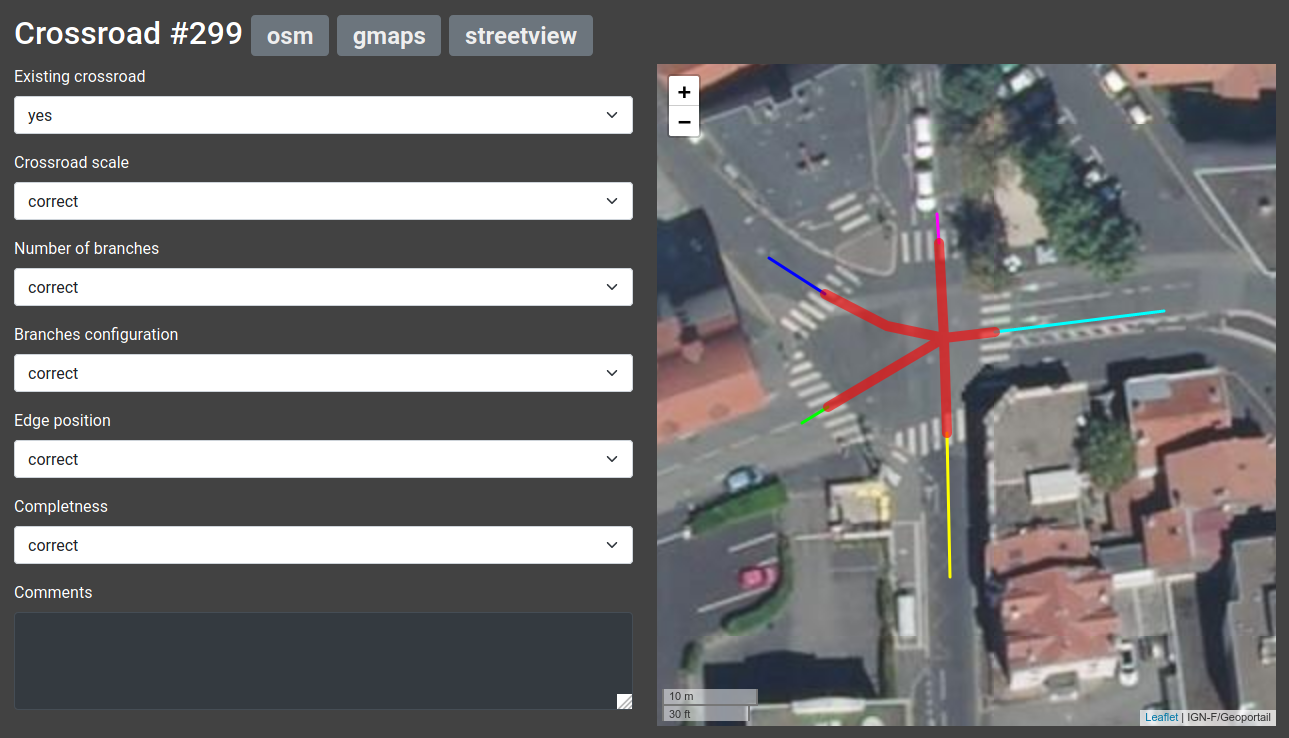
\includegraphics[width=0.75\textwidth]{images/evaluation/evaluation-xxx.png}
    \caption[Interface de l'outil d'évaluation]{Interface de l'outil d'évaluation. Source: \citep{Favreau2022}.}
    \label{fig:evaluationTool}
\end{figure}

\newpar{}

L'outil génère un fichier d'évaluation pour chaque zone d'intérêt, qui peut être exploré à l'aide d'une interface dédiée (figure~\ref{fig:explorer}), afin d'avoir un aperçu synthétique du résultat de l'algorithme dans la zone considérée.

\begin{figure}[ht]
    \centering
    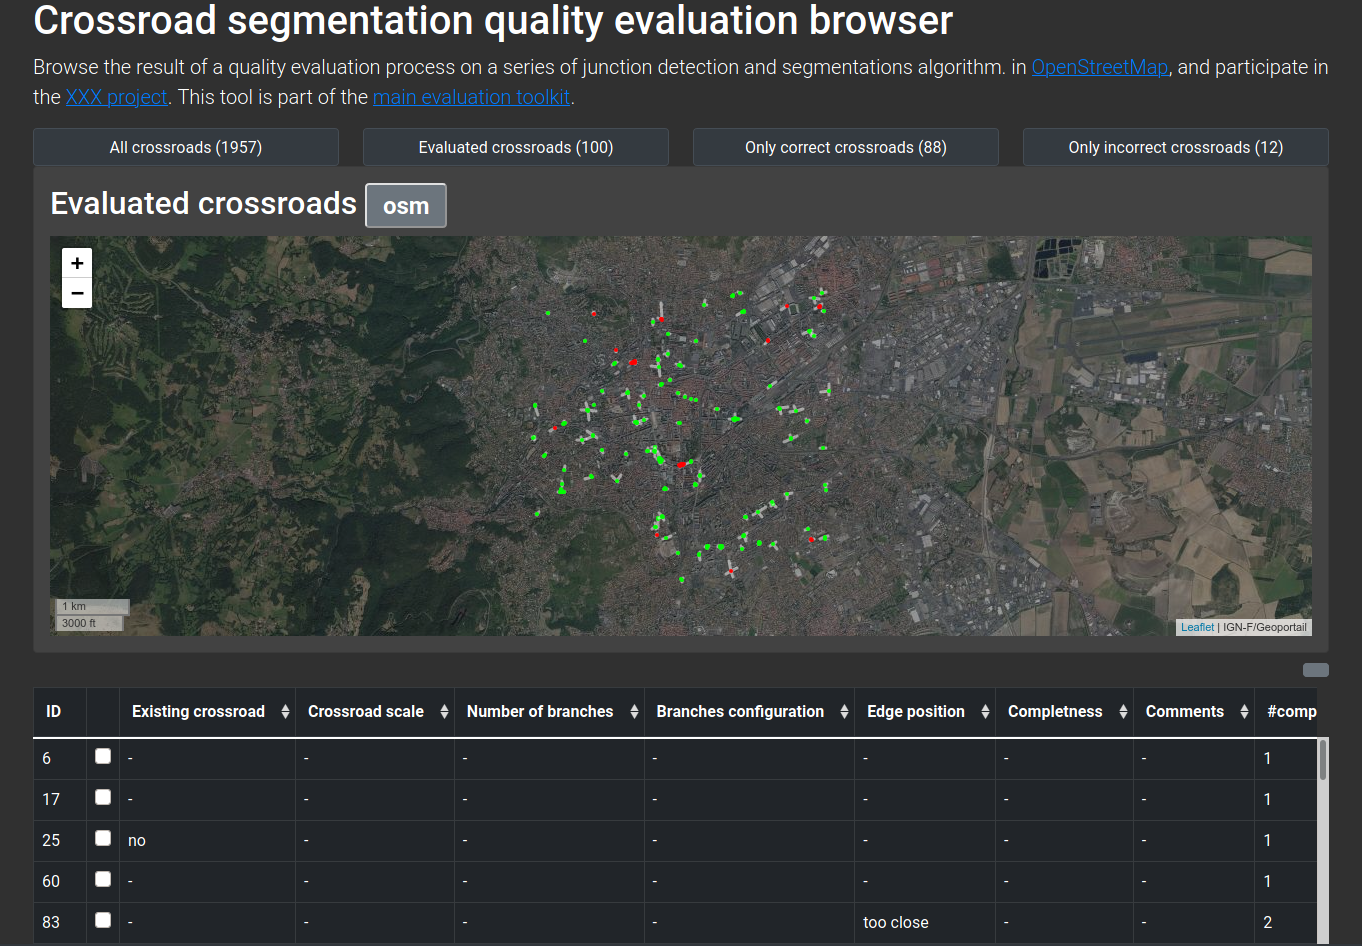
\includegraphics[width=0.75\textwidth]{images/evaluation/eval-browser-xxx.png}
    \caption[Interface pour explorer les évaluations réalisées]{Interface pour explorer les évaluations réalisées. Source: \citep{Favreau2022}.}
    \label{fig:explorer}
\end{figure}

\subsection{Évaluation de crseg}

Pour l'évaluation statistique, nous avons sélectionné trois villes de taille représentative des villes françaises: la ville 1 (Paris, 10 785 092 habitants dans l'aire urbaine), la ville 2 (Nantes, 650 081 habitants dans l'aire urbaine) et la ville 3 (Clermont-Ferrand, 268 696 habitants dans l'aire urbaine). Sur chacune d'entre elles, nous avons sélectionné un point et récupéré toutes les données \gls{osm} dans un rayon de deux kilomètres autour de ce point (voir figure~\ref{fig:regions}).

\begin{figure}[H]
    \centering
    \begin{subfigure}[t]{0.32\linewidth}
        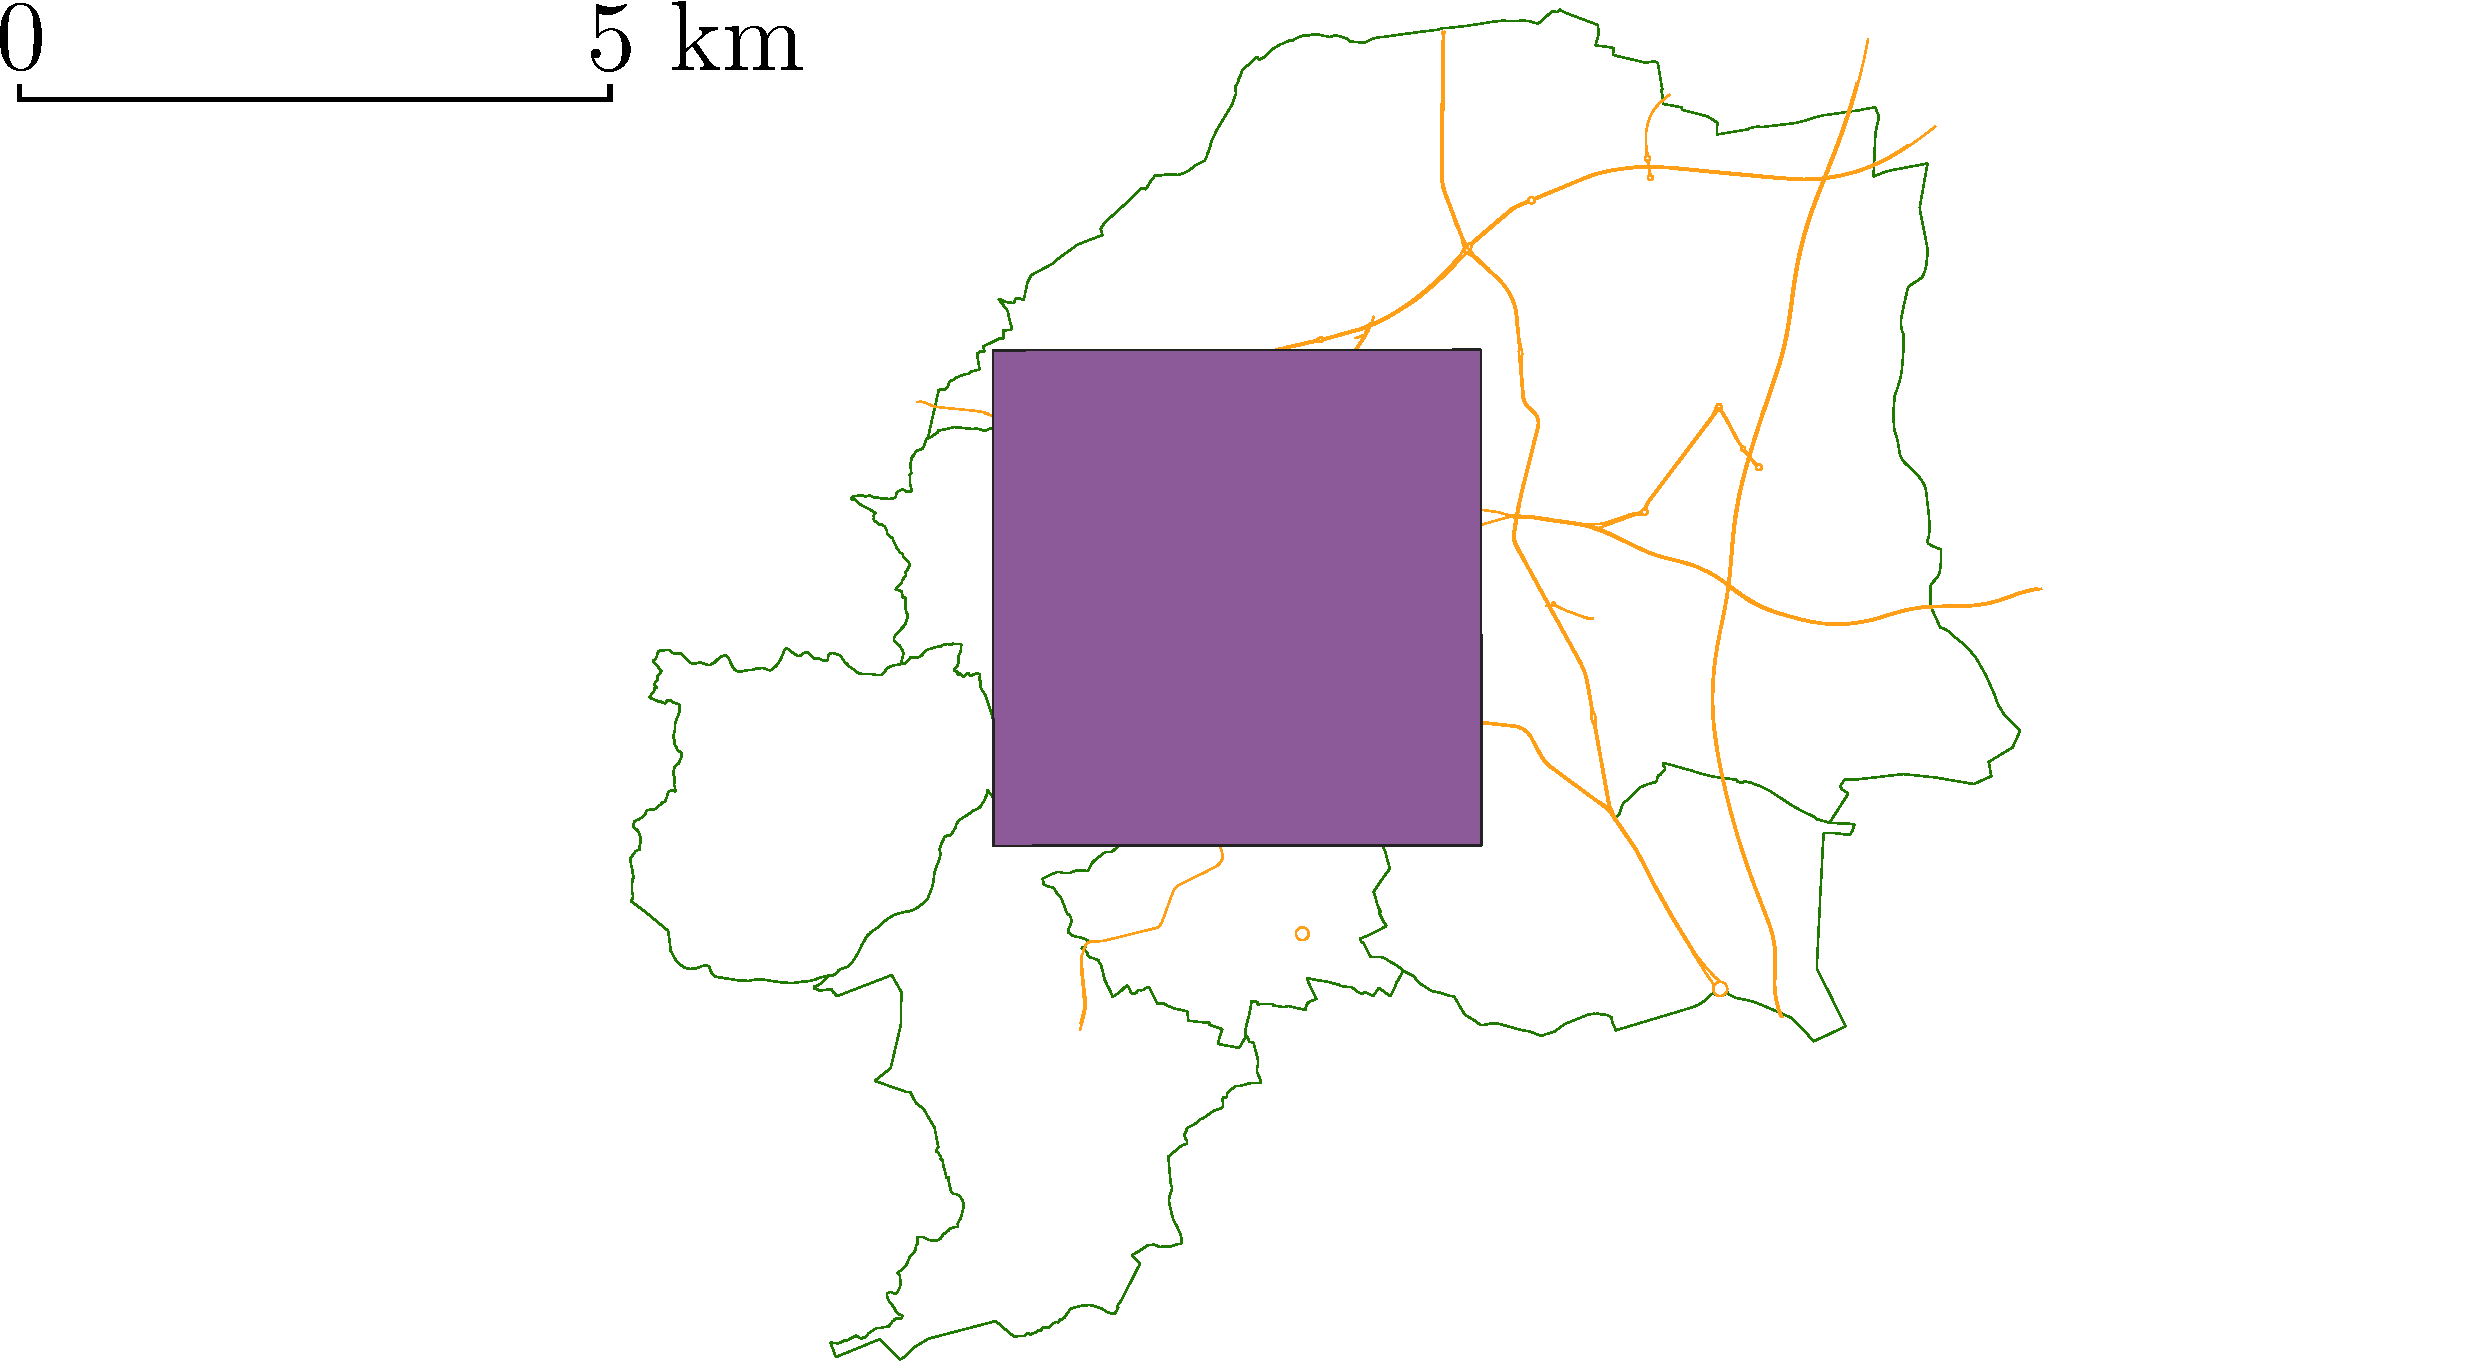
\includegraphics[width=\textwidth]{images/evaluation/crseg/clermont.pdf}
        \caption{}
        \label{fig:clermontRegion}
    \end{subfigure}
    \hfill
    \begin{subfigure}[t]{0.32\linewidth}
        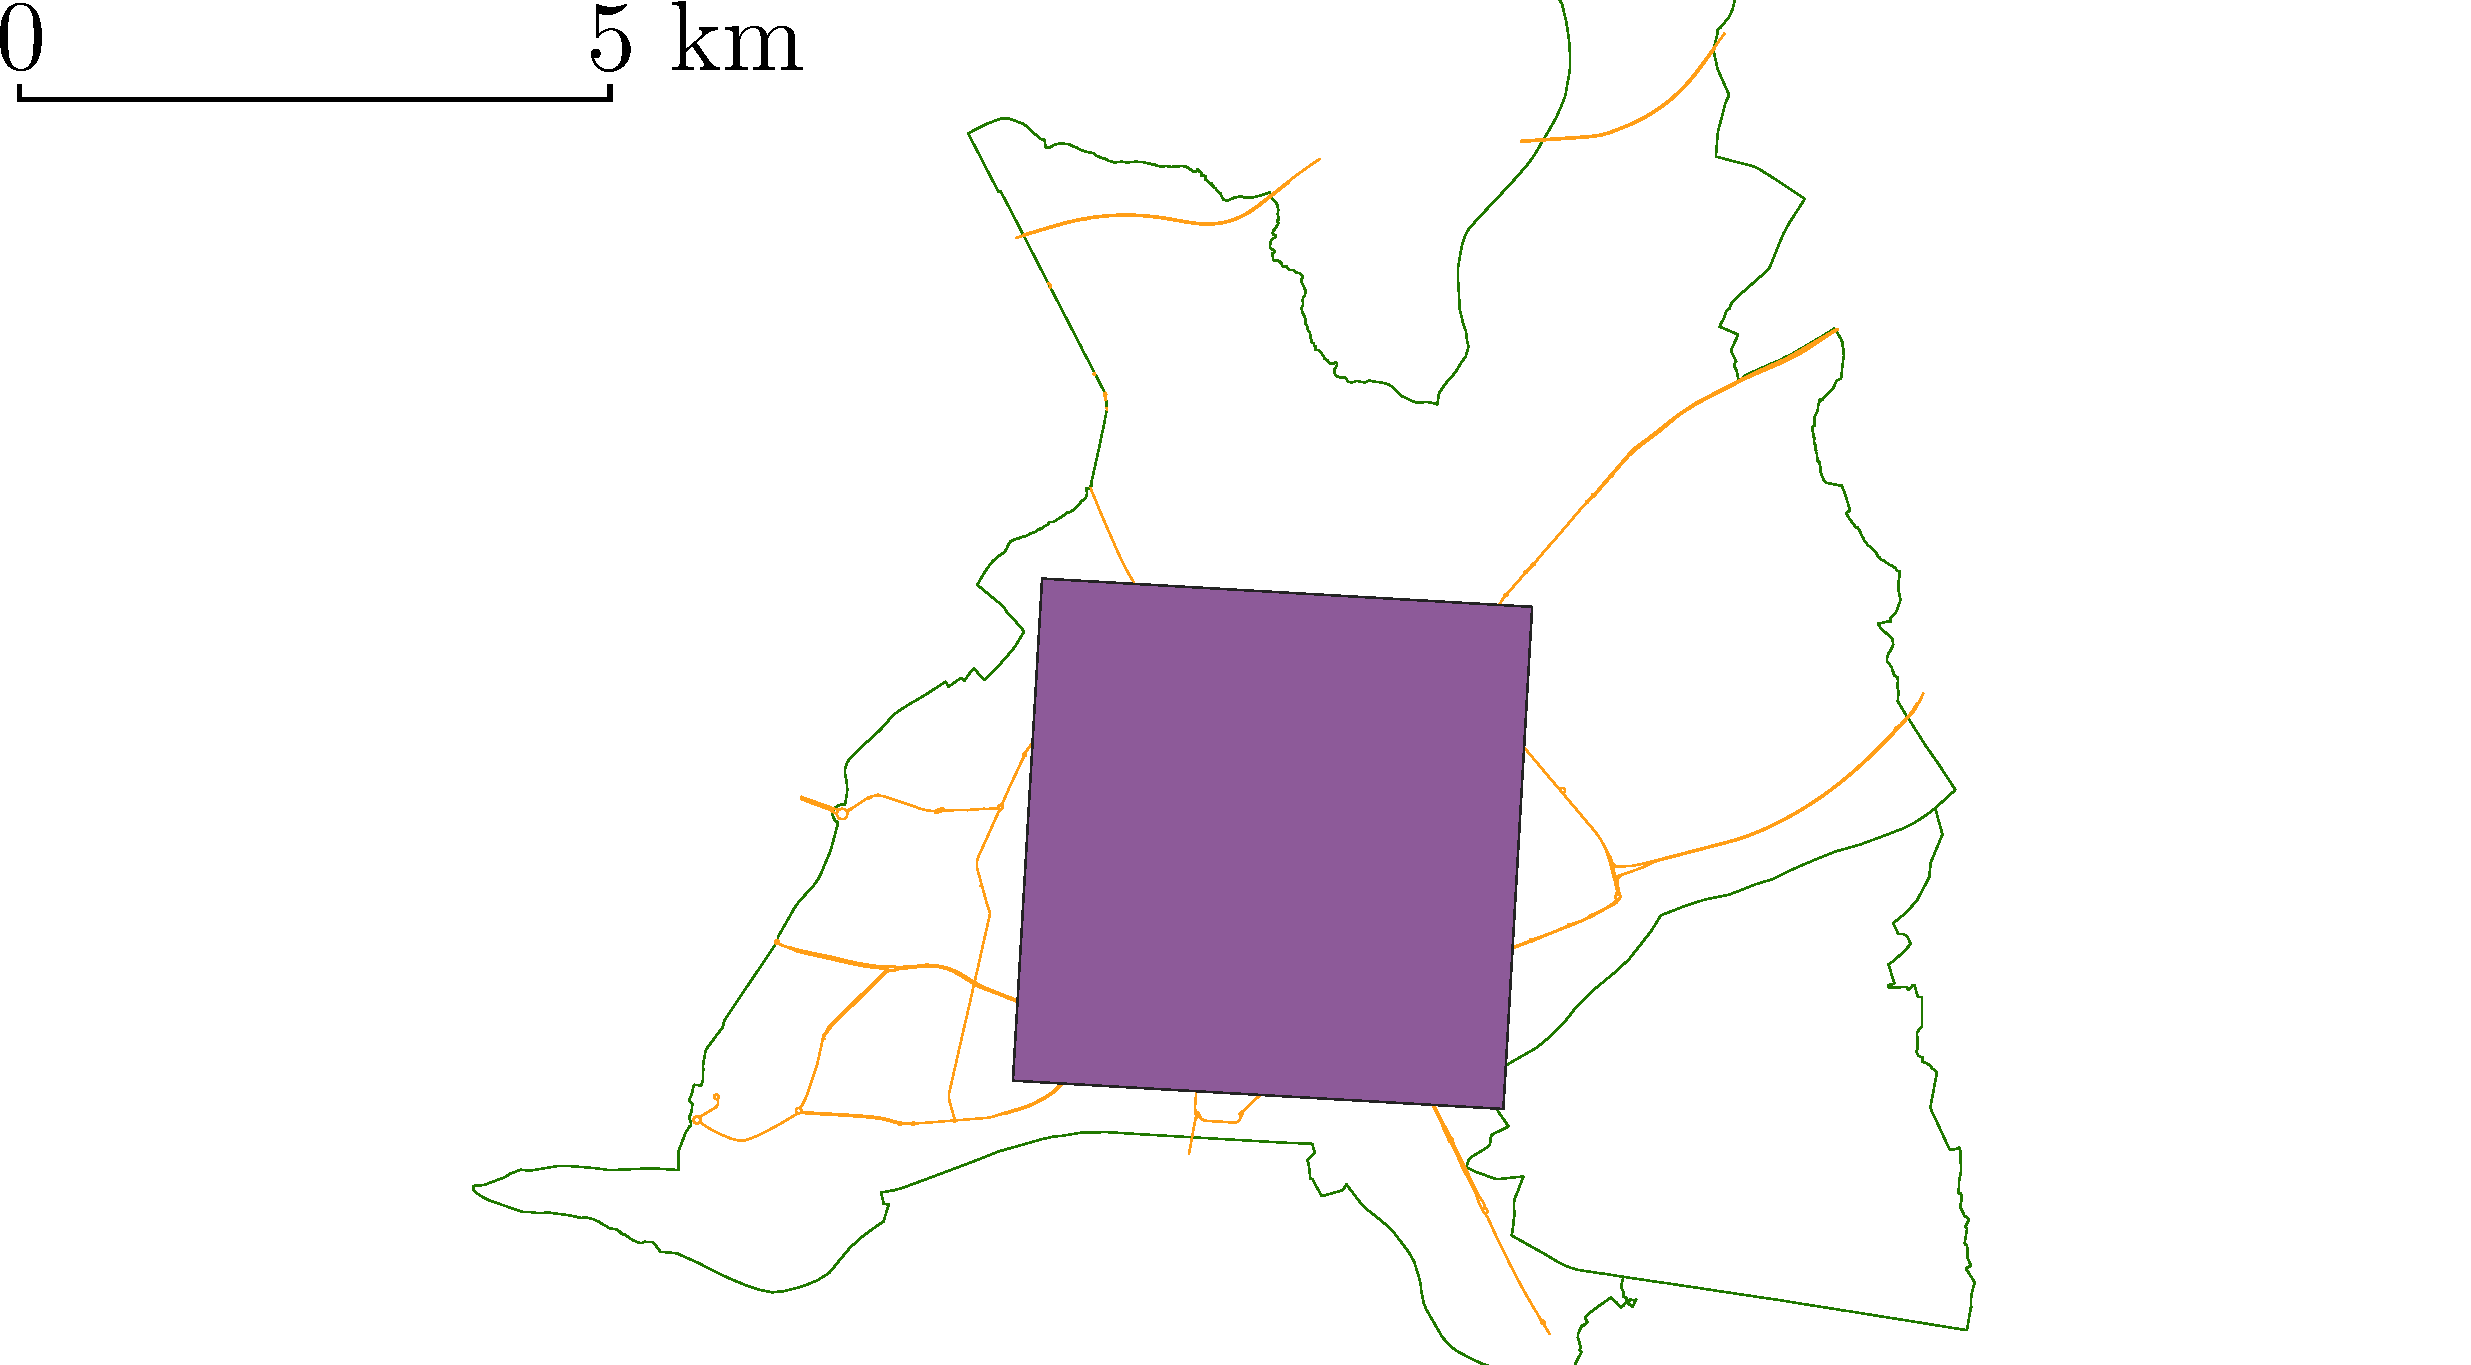
\includegraphics[width=\textwidth]{images/evaluation/crseg/nantes.pdf}
        \caption{}
        \label{fig:nantesRegion}
    \end{subfigure}
    \begin{subfigure}[t]{0.32\linewidth}
        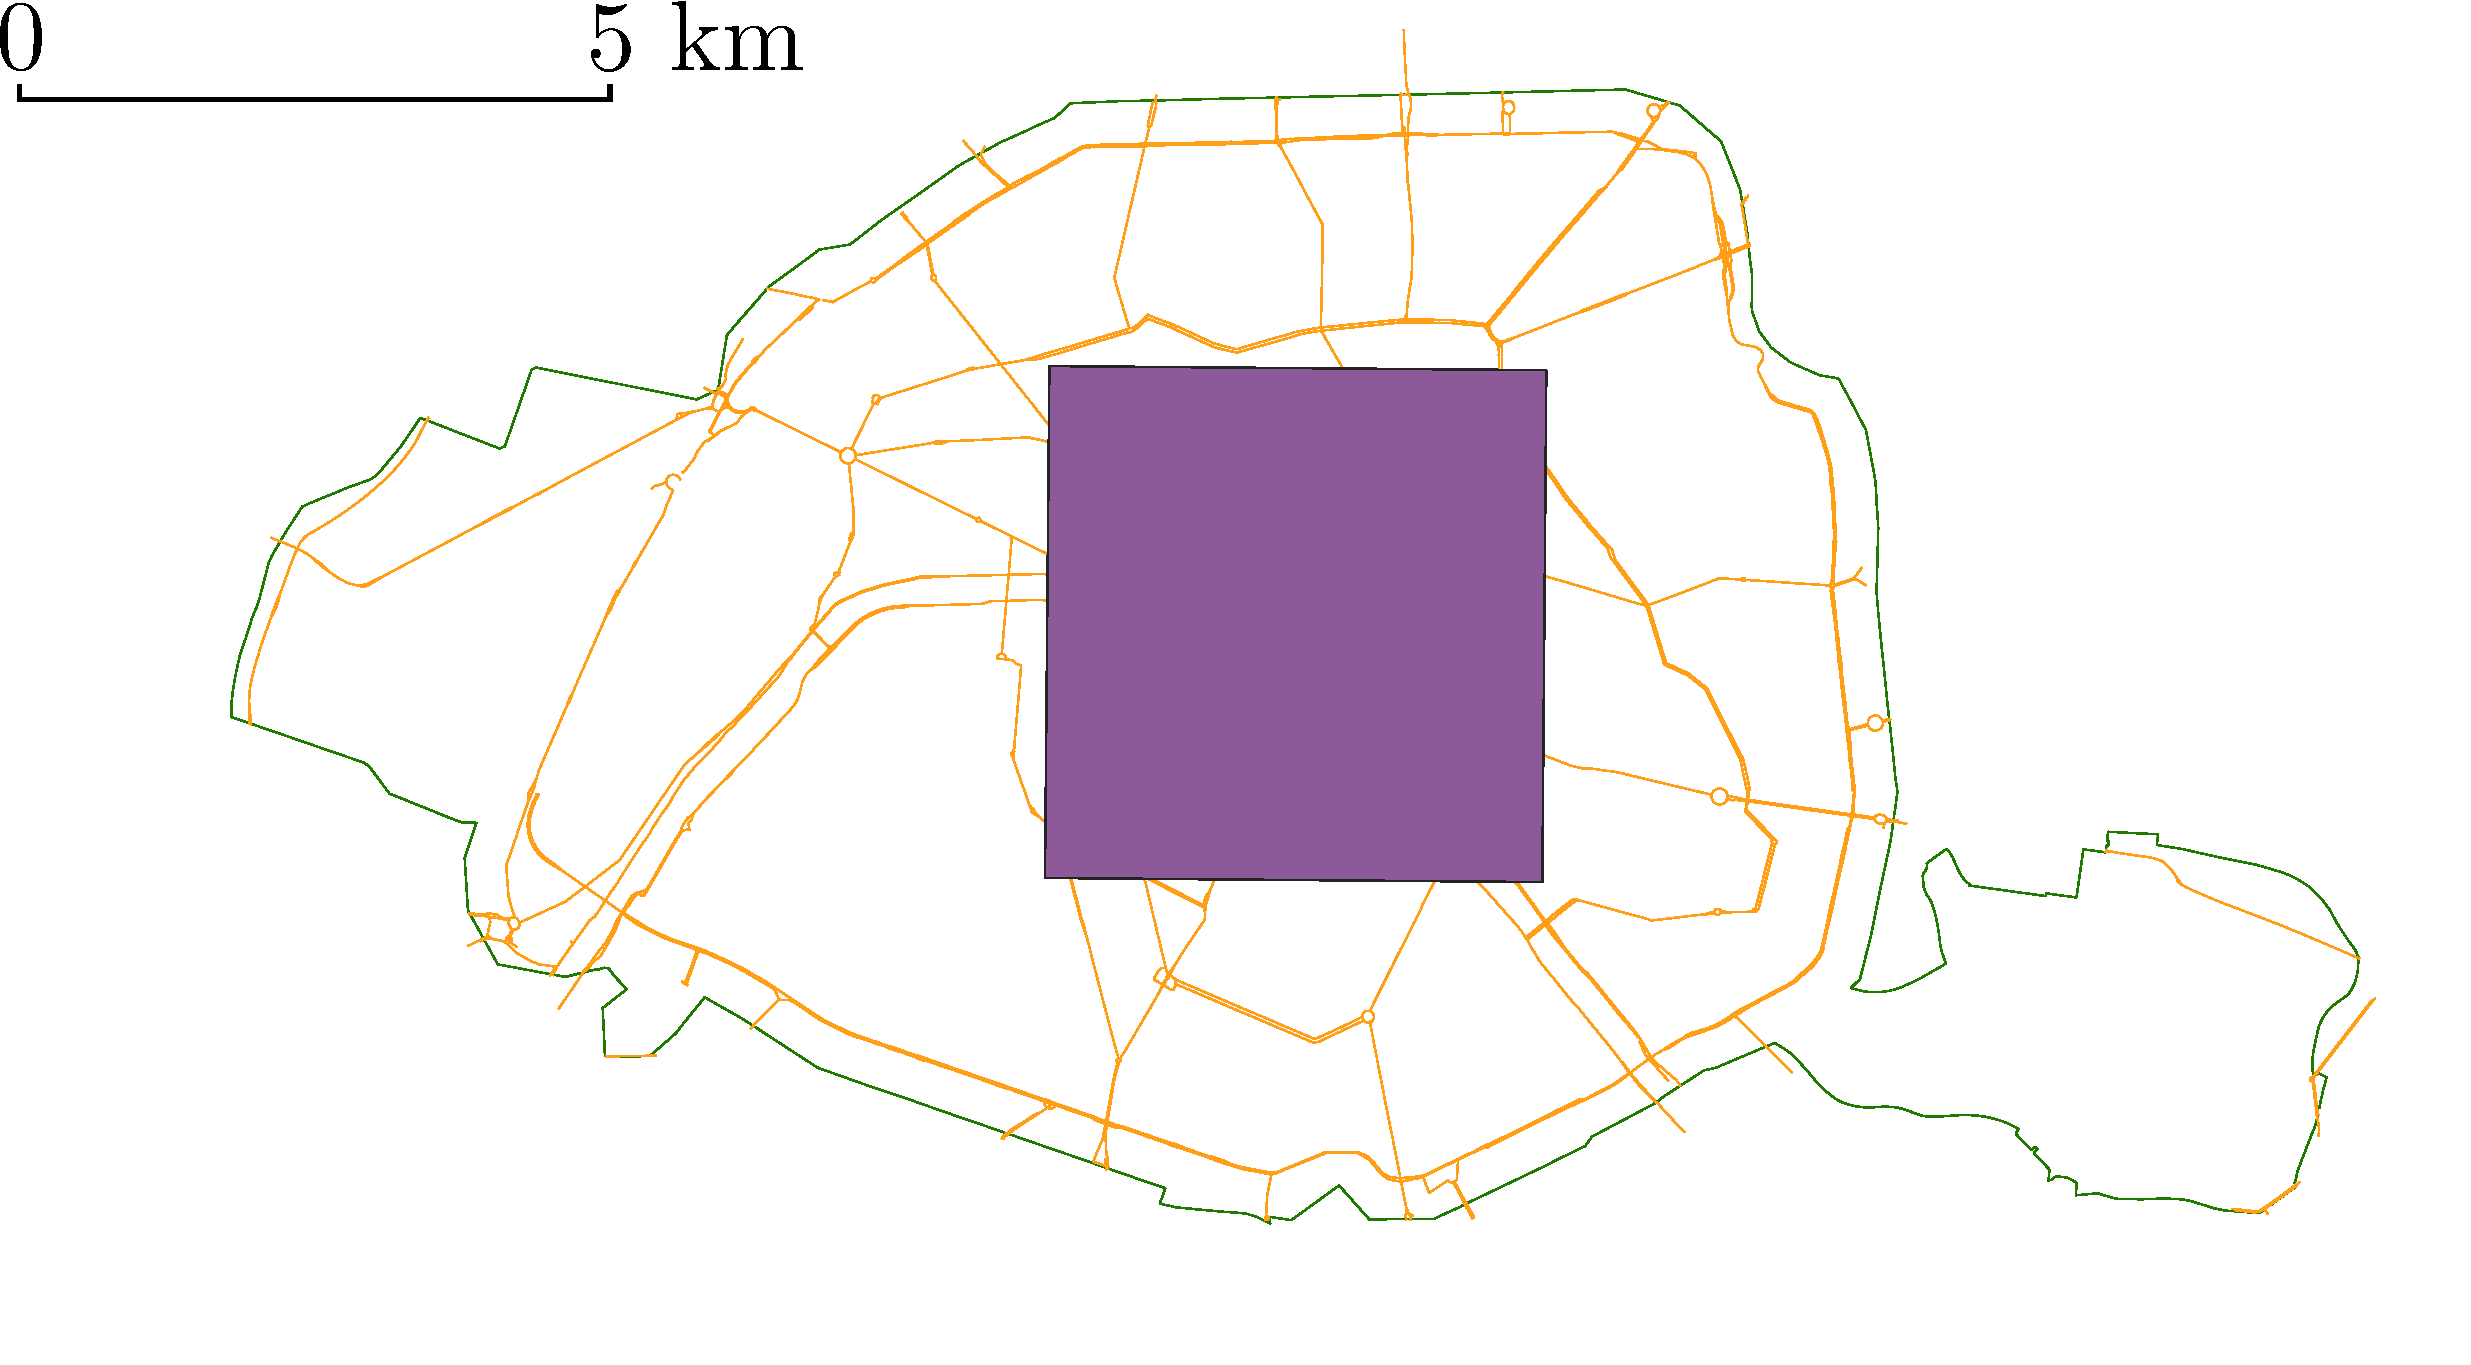
\includegraphics[width=\textwidth]{images/evaluation/crseg/paris.pdf}
        \caption{}
        \label{fig:parisRegion}
    \end{subfigure}
    \caption[Régions sélectionnées pour l'évaluation statistique]{Régions sélectionnées pour l'évaluation statistique. La région (a) contient des rues qui font partie des villes suivantes: Clermont-Ferrand, Aubière, Beaumont, Ceyrat, Royat et Chamalières. La région (b) contient des rues qui font partie de Nantes et Saint-Sébastien sur Loire. La région (c) est centrée sur Paris. Source: \citep{Favreau2022}.}
    \label{fig:regions}
\end{figure}

\pagebreak

Nous avons appliqué le processus de segmentation sur chacune des régions, obtenant un total de 5 553 carrefours. Le tableau~\ref{tab:initRegions} donne pour chaque région la répartition des carrefours selon leur complexité: simple, intermédiaire ou complexe (voir figure \ref{fig:carrefours_simple_intermediaire_complexe}). 

\begin{table}[ht] 
    \centering
    \footnotesize
    \begin{tabular}{c|c|c|c|c}
    Région & \#total & \#simple &\#intermédiaire & \#complexe \\
    \hline
     1 & 1,818 & 265 & 1,541  & 12 \\
     2 & 1,778 & 573 & 1,190 & 15 \\
     3 & 1,957 & 1,006 & 931  & 20 \\
     \hline
     toutes & 5,553  & 1,844 & 3,662 &	47  \\
     \hline
     ratio & & 33.2\% & 65.9\% & 0.8\% \\
    \end{tabular}
    \caption[Complexité des carrefours générés dans chaque région]{Complexité des carrefours générés dans chaque région. Source: \citep{Favreau2022}.}
    \label{tab:initRegions}
\end{table}

\begin{figure}[ht]
    \centering
    \begin{subfigure}[t]{.25\linewidth}
        \centering
        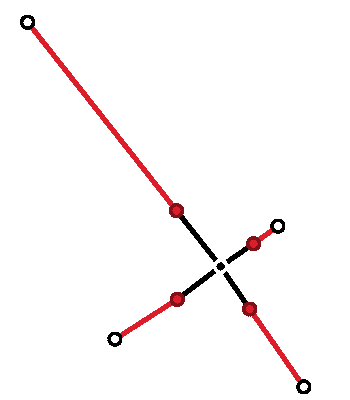
\includegraphics[width=\linewidth]{images/evaluation/crseg/carrefour_simple.pdf}
        \caption{}
    \end{subfigure}
    \begin{subfigure}[t]{.25\linewidth}
        \centering
        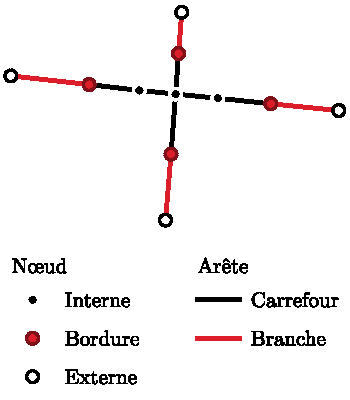
\includegraphics[width=\linewidth]{images/evaluation/crseg/carrefour_intermediaire.pdf}
        \caption{}
    \end{subfigure}
    \begin{subfigure}[t]{.25\linewidth}
        \centering
        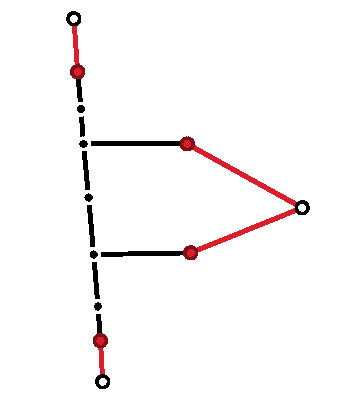
\includegraphics[width=\linewidth]{images/evaluation/crseg/carrefour_complexe.pdf}
        \caption{}
    \end{subfigure}
    \caption[Typologie des complexités de carrefour]{Typologie des complexités de carrefour considérée pour l'évaluation: les carrefours simples (a) ont un seul nœud interne, les carrefours intermédiaires (b) ont plusieurs nœuds internes dont un seul a une cardinalité supérieure à 2 et les carrefours complexes (c) ont plusieurs nœuds internes de cardinalité supérieure à 2.}
    \label{fig:carrefours_simple_intermediaire_complexe}
\end{figure}

\newpar{}

Nous avons utilisé l'outil d'évaluation présenté dans la partie \ref{sec:evaluation_implementation}. En jouant nous même le rôle de l'expert, nous avons évalué 100 carrefours dans chaque région, sélectionnés aléatoirement. Le tableau~\ref{tab:selectedRegions} montre que la répartition des carrefours en fonction de leur complexité est comparable à celle de toutes les régions. 

\begin{table}[ht]
    \centering
    \footnotesize
    \begin{tabular}{c|c|c|c|c}
    Région & \#total & \#simple &\#intermédiaire& \#complexe \\
    \hline
     1 & 100 & 29 & 70 & 1 \\
     2 & 100 & 17 & 83 & 0 \\
     3 & 100 & 52 & 45 & 3 \\
     \hline
     toutes & 300 & 98 & 198 & 4 \\
     \hline
     ratio & &  32.7\% & 66\% & 1.3\%\\
    \end{tabular}
    \caption[Complexité des carrefours choisis au hasard]{Complexité des carrefours choisis au hasard. Source: \citep{Favreau2022}.}
    \label{tab:selectedRegions}
\end{table}

\newpar{}

Nous avons défini les critères d'évaluation suivants:
\begin{itemize}
    \item Carrefour existant: \textit{oui} ou \textit{non},
    \item Échelle du carrefour: \textit{correcte}, \textit{trop grande} ou \textit{trop petite},
    \item Nombre de branches: \textit{correct}, \textit{trop peu} ou \textit{trop nombreuses},
    \item Configuration des branches: \textit{correcte}, \textit{deux branches ou plus sont fusionnées}, \textit{une branche ou plus sont divisées} ou \textit{branches fusionnées et divisées},
    \item Position des bordures (relatif au centre du carrefour): \textit{correctes}, \textit{trop proches} ou \textit{trop éloignées},
    \item Complétude: \textit{correcte}, \textit{parties manquantes} ou \textit{parties en trop}.
\end{itemize}

\newpar{}

Deux exemples d'erreurs de segmentation sont illustrés en figure~\ref{fig:eval_ex_err_crseg}.

\begin{figure}[ht]
    \centering
    \begin{subfigure}[t]{.4\linewidth}
        \centering
        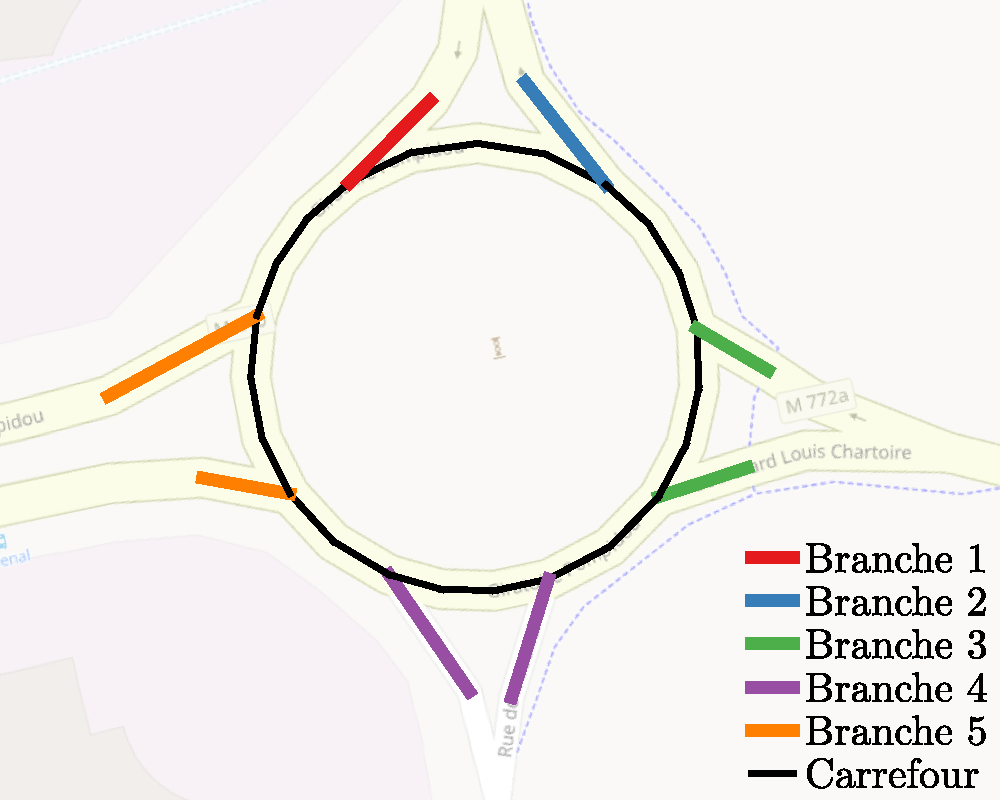
\includegraphics[width=\linewidth]{images/evaluation/crseg/crseg_err_branches.pdf}
        \caption{}
    \end{subfigure}
    \begin{subfigure}[t]{.4\linewidth}
        \centering
        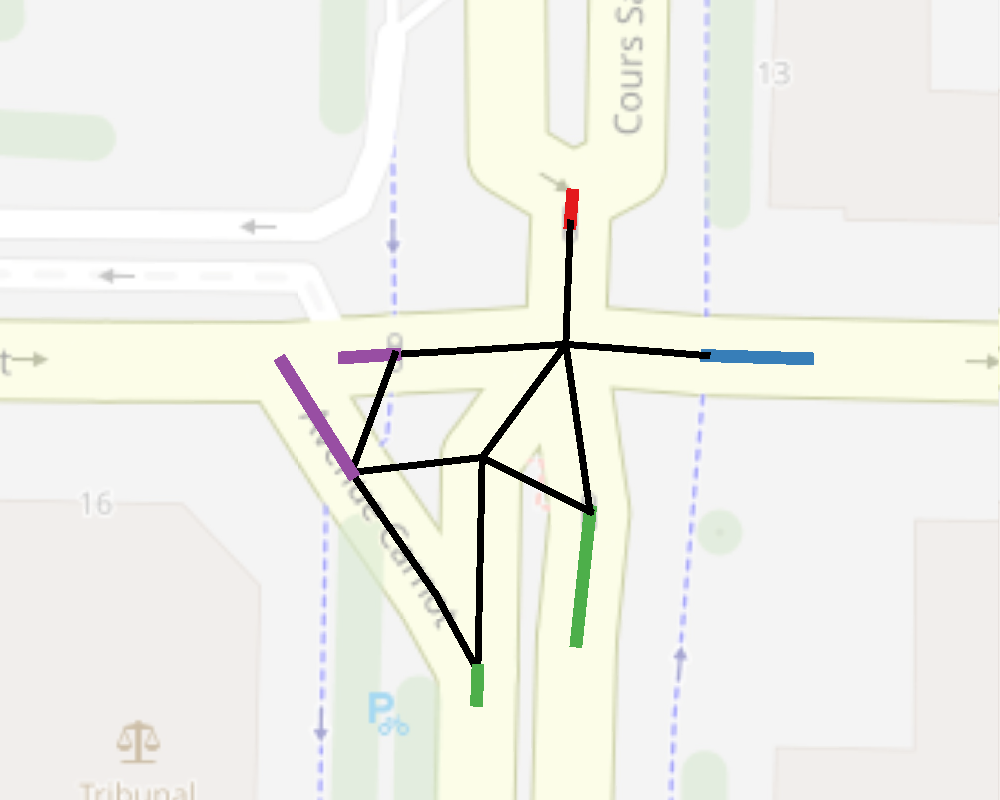
\includegraphics[width=\linewidth]{images/evaluation/crseg/crseg_err_manquant.pdf}
        \caption{}
    \end{subfigure}
    \caption[Exemples d'erreurs de segmentation]{Exemples d'erreurs de segmentation. (a) Les branches 1 et 2 sont séparées alors qu'il s'agit d'une même branche. Cette erreur est due à l'absence de nom de voie sur ces deux tronçons dans les données \gls{osm}. (b) La contre-allée qui part du nord et se dirige vers l'ouest est manquante. Cette configuration avec une contre-allée déconnectée du carrefour n'est pas prise en compte par notre algorithme.}
    \label{fig:eval_ex_err_crseg}
\end{figure}

\newpar{}

Sur ces 300 carrefours, 245 ont été validés par les critères évoqués précédemment en comparant la segmentation avec l'orthophotographie proposée par l'interface (voir table~\ref{tab:nbRegions}).

\newpar{}

\begin{table}[ht]    
    \centering
    \footnotesize
    \begin{tabular}{c|c|c|c}
         Région & \#total & \#sélectionné & \#segmentation valide \\
         \hline
         1 & 1,818 & 100 & 81 \\
         2 & 1,778 & 100 & 76 \\
         3 & 1,957 & 100 & 88 \\
    \end{tabular}
    \caption[Description du jeu de données d'évaluation]{Description du jeu de données: pour chaque région, le nombre de carrefours obtenus par notre algorithme, le nombre de carrefours sélectionnés aléatoirement (100), et le nombre de segmentations valides par rapport à l'orthophotographie. Source: \citep{Favreau2022}.}
    \label{tab:nbRegions}
\end{table}


Sur les 55 carrefours restants, 26 sont affectés par un problème d'ajustement des limites, l'orthophotographie montrant un passage piéton qui aurait dû être inclus dans la segmentation.
Après analyse, 11 carrefours sont concernés par des passages piétons manquants dans \gls{osm}, 3 carrefours par un passage piétons dépassé ou mal positionné, et 2 carrefours car une rue adjacente est une rue piétonne selon \gls{osm}, ce qui semble incorrect au regard de l'orthophotographie. Les 10 autres limites mal positionnées nécessiteraient un ajustement local du paramètre C0.

\newpar{}

Parmi les carrefours restants, 21 ont été considérés comme ayant des parties manquantes ou comme étant à une échelle trop grande ou trop petite. Il y a plusieurs causes à cela: 
\begin{itemize}
    \item pour 2 d'entre eux, il s'agit d'une voie manquante dans la modélisation \gls{osm}, 
    \item pour 3 autres, une rue adjacente a été identifiée dans \gls{osm} comme n'étant pas accessible aux voitures, 
    \item pour 4 autres, il s'agit de routes bordant ou entrant dans une place, espaces non pris en compte par l'algorithme,
    \item pour 12 d'entre eux, l'ajustement local du paramètre C1 ou C2 aurait permis de corriger la segmentation.
\end{itemize}

\newpar{}

Deux carrefours ont été considérés comme inexistants. Après analyse, il s'agissait d'approximations dans la modélisation \gls{osm} (voie privée mal étiquetée, modélisation inexacte d'un passage piéton linéaire).

\newpar{}

L’un des carrefours avait ses trois branches combinées en une seule. L'algorithme n'a pas interprété correctement un carrefour en T dans un quartier résidentiel où chaque branche portait le même nom.

\newpar{}

L’un des carrefours a vu l’une de ses branches divisée en deux branches. Après analyse, ces deux voies correspondaient à la desserte d'un parking et n'avaient pas de nom, ce qui empêchait l'algorithme de les associer.

\newpar{}

Enfin, nous avons également identifié un carrefour situé au milieu d'un parc, et 3 carrefours au milieu de parkings, ce qui invite à un travail plus poussé sur le filtrage des données \gls{osm}.

\newpar{}

En résumé (figure~\ref{fig:camembert}), la segmentation de 23 carrefours peut être corrigée en ajustant localement l'un des trois paramètres de la méthode, 18 carrefours sont imprécis en raison de l'absence ou de l'imprécision des données dans \gls{osm}, et 14 carrefours illustrent le manque de généralité de notre algorithme, qui ne prend pas en compte les voies fermées aux voitures, les voies sans nom, les carrefours ayant le même nom sur toutes les branches, ou encore le contexte (place, parc, parking).

\begin{figure}[ht]
    \centering
    \footnotesize
    \begin{tikzpicture}
        \pie[color = {
        blue!60, 
        blue!45, 
        gray, orange}]{81.6/A, 6/B, 4.6/C, 7.7/D}
    \end{tikzpicture}
    \caption[Répartition des carrefours considérés lors du processus d'évaluation]{Répartition des carrefours considérés lors de notre processus d'évaluation (table~\ref{tab:nbRegions}) en fonction de leur typologie. A (245 carrefours): segmentation correspondant à l'orthophotographie, B (18 carrefours): manque ou imprécision dans \gls{osm}, C (14 carrefours): régions non supportées, D (23 carrefours): nécessite un ajustement local des paramètres. Source: \citep{Favreau2022}.}
    \label{fig:camembert}
\end{figure}

\subsection{Évaluation de crmodel}

L'évaluation de l'implémentation de crmodel permet d'estimer sa capacité à générer des descriptions satisfaisantes au regard des données disponibles dans OpenStreetMap. Nous avons choisi de réaliser l'évaluation sur trois villes françaises: Lyon (522 969 habitants), Clermont-Ferrand (147 865 habitants) et Brive-la-Gaillarde (46 330 habitants).

\newpar{}

La qualité de la description a été évaluée en fonction de sa conformité avec le terrain et les données disponibles. Une description définie comme correcte correspond au terrain. Une description partiellement correcte indique qu'elle correspond en partie au terrain mais que les données, l'implémentation ou la segmentation étaient insuffisantes pour fournir une description complète. Une description incorrecte ne correspond pas du tout au terrain. Des descriptions de 20 carrefours par ville, choisis au hasard, ont été générées et l'instanciation des branches et des traversées a été évaluée. L'évaluation est basée sur l'outil proposé par en partie \ref{sec:evaluation_implementation}. Les valeurs des attributs OpenStreetMap ont été confrontées aux images aériennes afin d'évaluer les problèmes de données. Les dispositifs sonores des passages piétons n'ont pas été pris en compte car les images aériennes ne permettent pas de vérifier cette information. Nous avons défini les critères d’évaluation suivants:
\begin{itemize}
    \item Première branche au nord: \textit{oui}, \textit{non} ou \textit{indéfini}
    \item Présence des voies sur \gls{osm}: \textit{corrects}, \textit{attributs manquants} ou \textit{objets manquants},
    \item Nombre de voies: \textit{correct}, \textit{trop peu} ou \textit{trop nombreuses},
    \item Types de voies: \textit{corrects}, \textit{incorrects},
    \item Ordre des voies: \textit{corrects}, \textit{incorrects},
    \item Présence des passages piétons sur \gls{osm}: \textit{corrects}, \textit{attributs manquants} ou \textit{objets manquants},
    \item Génération des traversées: \textit{correctes}, \textit{incorrectes}, \textit{trop peu} ou \textit{trop nombreuses}
\end{itemize}

\newpar{}

Trois cas dans lesquels crmodel produit un résultat erroné sont illustrés en figure~\ref{fig:eval_ex_err_crmodel}.

\begin{figure}[ht]
    \centering
    \begin{subfigure}[t]{.3\linewidth}
        \centering
        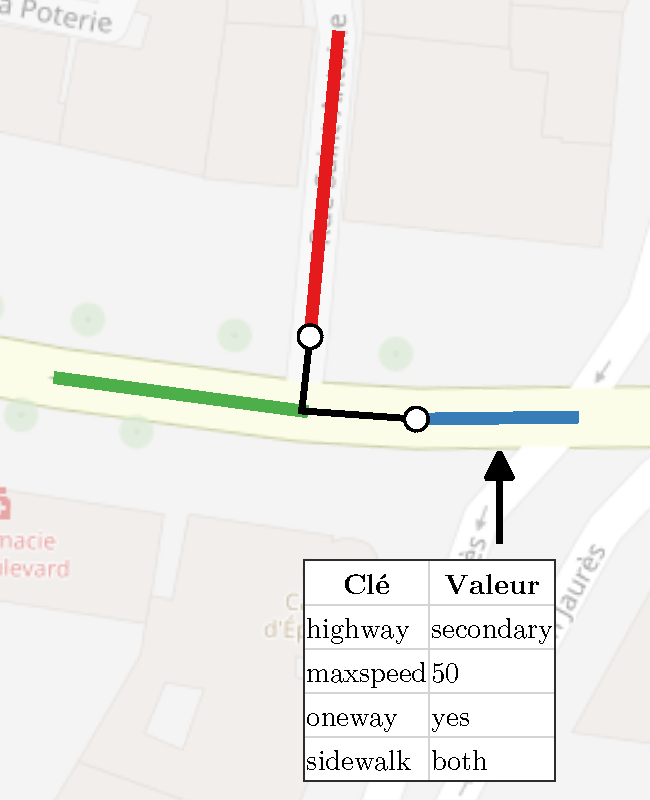
\includegraphics[width=\linewidth]{images/evaluation/crmodel/eval_cas1.pdf}
        \caption{}
    \end{subfigure}
    \begin{subfigure}[t]{.3\linewidth}
        \centering
        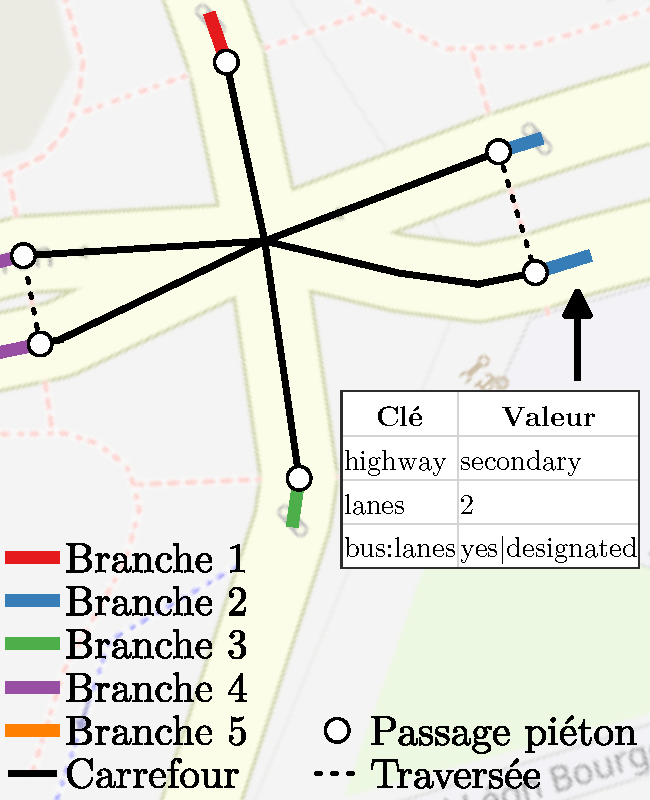
\includegraphics[width=\linewidth]{images/evaluation/crmodel/eval_cas2.pdf}
        \caption{}
    \end{subfigure}
    \begin{subfigure}[t]{.3\linewidth}
        \centering
        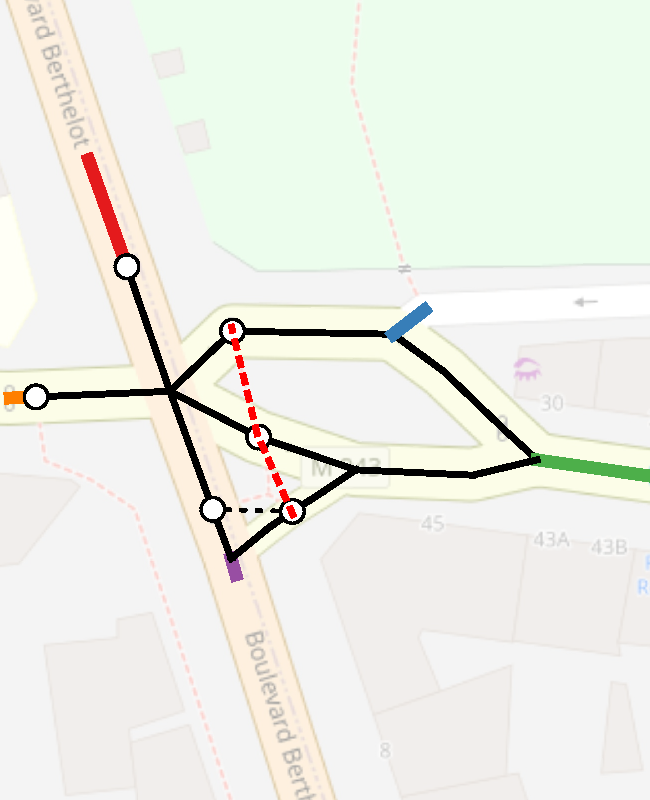
\includegraphics[width=\linewidth]{images/evaluation/crmodel/eval_cas3.pdf}
        \caption{}
    \end{subfigure}
    \caption[Exemples de résultats erronés de crmodel]{Exemples de cas où crmodel produit un résultat erroné. (a) les données \gls{osm} ne contiennent pas les attributs nécessaires pour décrire les voies et leur agencement. (b) La clé \osmkey{bus:lanes} qui permet d'indiquer le nombre de voies de bus n'est pas prise en compte par crmodel (la clé \osmkey{psv:lanes} est habituellement utilisée). (c) crmodel ne gère les traversées que par branche. Dans ce cas, les branches 2 et 3 se traversent simultanément en passant par l'îlot, donc crmodel ne génère pas la traversée (ici en traitillés rouges).}
    \label{fig:eval_ex_err_crmodel}
\end{figure}


\begin{figure}[ht]
    \centering
    \begin{tikzpicture}
        \pie[color = {
        blue!60, 
        blue!45, 
        gray}]{53.7/A, 14.8/B, 31.5/C}
    \end{tikzpicture}
    \caption[Types de problèmes rencontrés au cours du processus d'évaluation]{Distribution des types de problèmes rencontrés au cours du processus d'évaluation. A (29 carrefours): objets ou attributs manquants dans OpenStreetMap, B (8 carrefours): problèmes d'implémentation, soit des attributs non supportés, soit des erreurs d'algorithme, C (17 carrefours): erreurs mélangeant l'implémentation, la segmentation et les problèmes de données.}
    \label{fig:camissues}
\end{figure}

\newpar{}

La description du nombre et des noms des branches est celle qui donne les meilleurs résultats. Ceux-ci dépendent principalement de la qualité de la segmentation (19 intersections sur 20, soit 95\% des erreurs rencontrées). Les descriptions des voies des branches et les descriptions des traversée sont plus sensibles à la qualité des données OpenStreetMap (respectivement 26 sur 41 et 30 sur 36 intersections, soit 63,4\% et 83,3\% des erreurs rencontrées). Les voies sont également fortement affectées par les erreurs d'implémentation (19 intersections sur 41, soit 46,3\% des erreurs rencontrées) car toutes les clés \gls{osm}, notamment celles relatives aux lignes de bus, n'ont pas été prises en compte.  Ces résultats sont résumés dans le tableau~\ref{tab:descqualitybydesctype}.

\begin{table}[ht]
    \begin{center}
        \footnotesize
        \begin{tabular}{ c | c | c | c }
            Qualité de la description & Nombre et noms des branches & Voies des branches & Traversées\\
            \hline
            Correct & 40  & 19 & 24 \\
            Partiellement correct & 17 & 40 & 34 \\
            Incorrect & 3 & 1 & 2 \\
            \hline
            Nombre de carrefours & 60 & 60 & 60
        \end{tabular}
        \caption[Qualité de la description par type de données]{Qualité de la description par type de données.}
        \label{tab:descqualitybydesctype}
    \end{center}
\end{table}

\newpar{}

Les résultats globaux indiquent que seuls 6 carrefours de l'échantillon ont été parfaitement décrits. D'autre part, 56 intersections ont été au moins partiellement décrites correctement. Le principal problème à l'origine de la dégradation de la description est la qualité des données \gls{osm} (figure~\ref{fig:camissues}) où les clés ou les objets manquants ont eu un impact sur la description. On peut cependant noter que les trois villes choisies n'ont pas la même qualité de données \gls{osm} (table~\ref{tab:osmqualityissues}).

\begin{table}[ht]
    \begin{center}
        \footnotesize
        \begin{tabular}{c | c | c | c }
            Type de problème & Lyon & Clermont-Ferrand & Brive-la-Gaillarde\\
            \hline
            Lié à \gls{osm} & 8  & 13 & 17 \\
            Non-lié à \gls{osm} & 9 & 4 & 3 \\
            \hline
            Nombre de problèmes & 17 & 17 & 20 \\
            Nombre de carrefours & 20 & 20 & 20
        \end{tabular}
        \caption[Relation entre les problèmes rencontrés et les données OpenStreetMap]{Problèmes rencontrés et leur relation avec les données \gls{osm} par ville.}
        \label{tab:osmqualityissues}
    \end{center}
\end{table}

\section{Évaluation du canevas de description}

Le canevas de conception de description décrit dans le chapitre \ref{chap:description} et implémenté dans le chapitre \ref{chap:implementation} a notamment été appliqué à la description de carrefours (voir partie \ref{sec:implementation_segmentation}). Dans cette partie, nous confrontons la description produite par notre chaîne à l'expertise des professionnels de la déficience visuelle pour déterminer les types de modifications qui pourraient être apportés au canevas. Puis nous évaluons la capacité de notre canevas à intégrer ces modifications.

\subsection{Enquête auprès des professionnels}

Le plan de description que nous avons présenté dans le chapitre \ref{chap:implementation} a été utilisé comme référence pour générer les description des carrefours. Cette description, bien qu'issue d'échanges avec des personne concernées ne répond pas nécessairement à la diversité des besoins exprimés par les utilisateurs. Pour évaluer sa correspondance avec les usages, et déterminer quels éléments pourraient être modulés, nous avons réalisé une enquête auprès de professionnels liés à la déficience visuelle.

\newpar{}

L'enquête a été réalisée avec l'outil en ligne LimeSurvey. Elle présente aux utilisateurs deux descriptions de carrefours générées par la chaîne présentée en partie \ref{sec:implementation_segmentation}. Les deux carrefours choisis et leurs descriptions associées sont illustrés en figure \ref{fig:evaluation_carrefours_enquete}. Pour chacun des carrefours, l'enquête présente une orthophotographie Google Satellite interactive centrée sur le carrefour et une vue immersive Google StreetView au même emplacement pour permettre aux participants de se familiariser avec le carrefour. Elle présente enfin la description du carrefour telle que générée par la chaîne présentée en partie \ref{sec:implementation_segmentation}, et invite les participants à modifier cette description pour l'adapter à leurs besoins et leurs pratiques. Il est à noter que les descriptions ont été générées le 8 juillet 2022.

\begin{figure}
    \begin{subfigure}[t]{\linewidth}
        \centering
        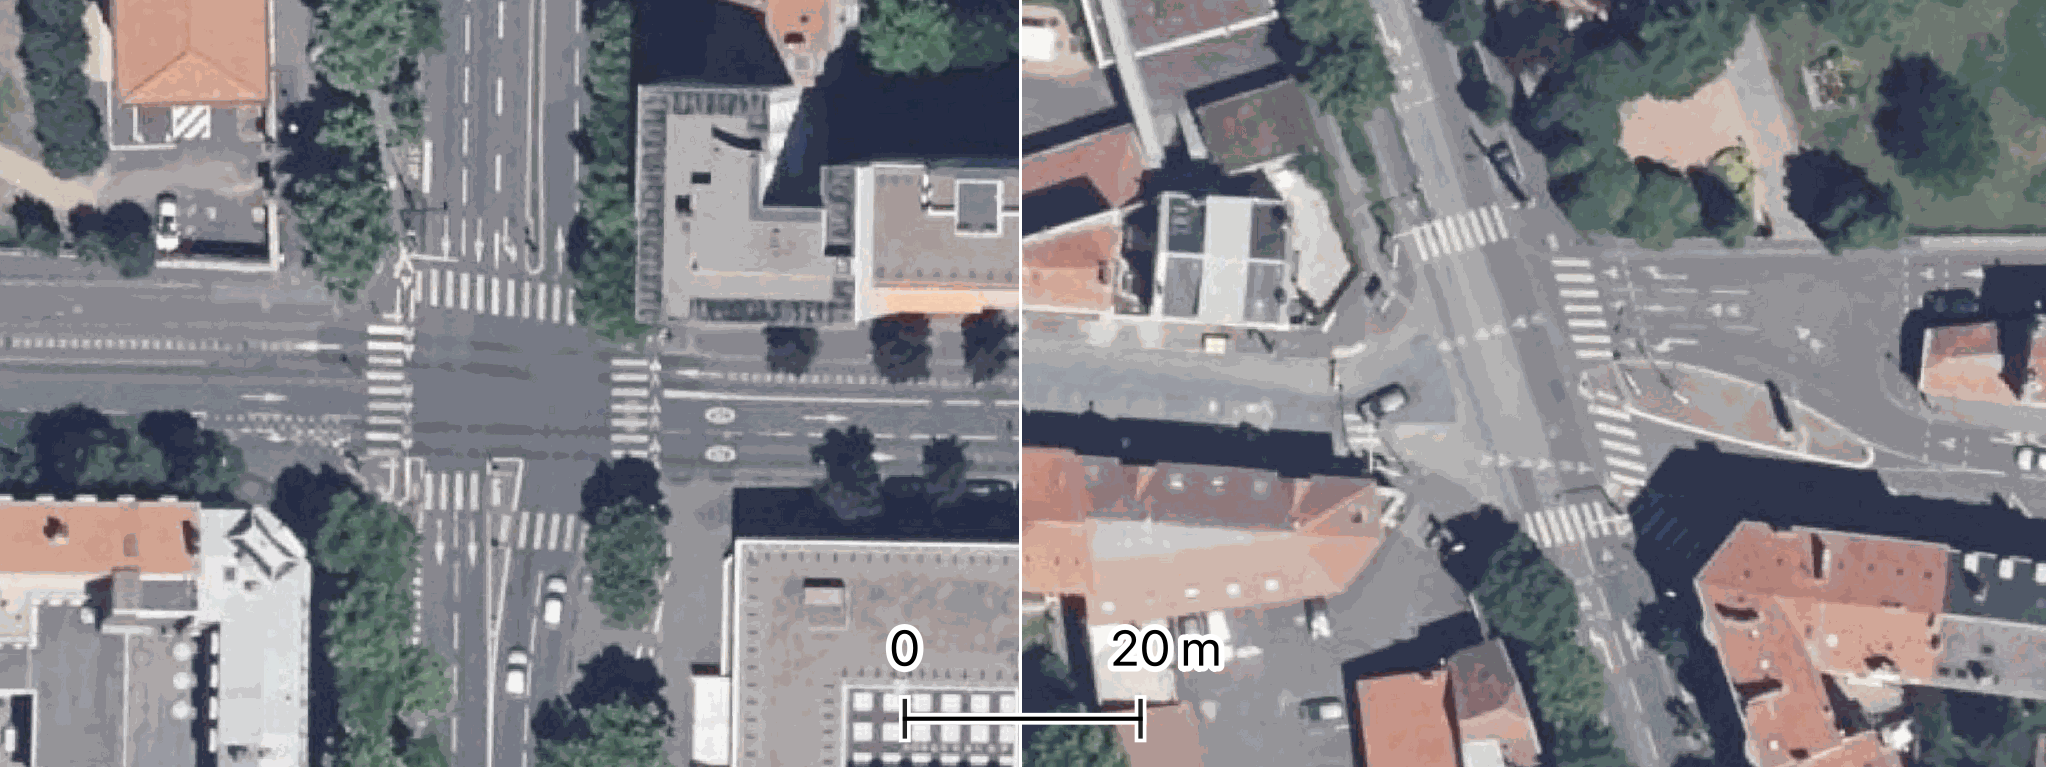
\includegraphics[width=\linewidth]{images/evaluation/ortho_carrefours_eval.png}
    \end{subfigure}
    \begin{subfigure}[t]{\linewidth}
        \centering
        \begin{minipage}[t]{0.49\linewidth}
            \vspace{0pt}
            \scriptsize
            Le carrefour à l'intersection du cours Sablon et de l'avenue Carnot est un carrefour à 4 branches.

            \vspace{5pt}

            La branche numéro un qui s'appelle cours Sablon est composée de trois voies de circulation sortantes, et deux voies de circulation entrantes.

            \vspace{5pt}

            La branche numéro deux qui s'appelle avenue Carnot est composée d'une voie de bus sortante, et une voie de circulation et une voie de bus entrante.

            \vspace{5pt}

            La branche numéro trois qui s'appelle cours Sablon est composée de deux voies de circulation sortantes, et deux voies de circulation entrantes.

            \vspace{5pt}

            La branche numéro quatre qui s'appelle avenue Carnot est composée de trois voies de circulation sortantes, et une voie de bus entrante.

            \vspace{5pt}

            La branche numéro un se traverse en deux fois. Les passages piétons sont tous protégés par un feu. Il y a des bandes d'éveil de vigilance.

            \vspace{5pt}

            La branche numéro deux se traverse en une fois. Les passages piétons sont tous protégés par un feu. Il y a des bandes d'éveil de vigilance.
            
            \vspace{5pt}

            La branche numéro trois se traverse en trois fois. Les passages piétons ne sont pas tous protégés par un feu. Il manque des bandes d'éveil de vigilance ou celles-ci sont dégradées.

            \vspace{5pt}

            La branche numéro quatre se traverse en trois fois. Les passages piétons ne sont pas tous protégés par un feu. Il manque des bandes d'éveil de vigilance ou celles-ci sont dégradées.
        \end{minipage}
        \begin{minipage}[t]{0.49\linewidth}
            \vspace{0pt}
            \scriptsize
            Le carrefour à l'intersection du boulevard Berthelot, de la rue Jean-Baptiste Torrilhon, de l'avenue Franklin Roosevelt et de l'avenue Joseph Claussat est un carrefour à 5 branches.

            \vspace{5pt}

            La branche numéro un qui s'appelle boulevard Berthelot est composée d'une voie de circulation sortante, et deux voies de circulation entrantes.

            \vspace{5pt}

            La branche numéro deux qui s'appelle rue Jean-Baptiste Torrilhon est composée d'une voie de circulation sortante.

            \vspace{5pt}

            La branche numéro trois qui s'appelle avenue Franklin Roosevelt est composée d'une voie de circulation entrante.

            \vspace{5pt}

            La branche numéro quatre qui s'appelle boulevard Berthelot est composée de deux voies de circulation sortantes, et une voie de circulation entrante.

            \vspace{5pt}

            La branche numéro cinq qui s'appelle avenue Joseph Claussat est composée d'une voie de circulation sortante, et deux voies de circulation entrantes.

            \vspace{5pt}

            La branche numéro un se traverse en une fois. Les passages piétons sont tous protégés par un feu. Il n'y a pas de bandes d'éveil de vigilance.

            \vspace{5pt}

            La branche numéro deux ne se traverse pas.

            \vspace{5pt}

            La branche numéro trois ne se traverse pas.

            \vspace{5pt}

            La branche numéro quatre se traverse en deux fois. Les passages piétons sont tous protégés par un feu. Il manque des bandes d'éveil de vigilance ou celles-ci sont dégradées.

            \vspace{5pt}
            
            La branche numéro cinq se traverse en une fois. Les passages piétons ne sont pas protégés par des feux. Il y a des bandes d'éveil de vigilance.
        \end{minipage}
    \end{subfigure}
    \caption[Carrefours choisis pour l'enquête auprès des instructeurs]{Les deux carrefours de Clermont-Ferrand choisis pour l'enquête présentent deux configurations différentes. Il s'agit dans les deux cas de carrefours complexes présentant des îlots et des particularités dans leurs cheminements. Source: BD Ortho IGN.}
    \label{fig:evaluation_carrefours_enquete}
\end{figure}

\newpar{}

L'enquête a démarré le 5 septembre 2022 et a été transmise au réseau national des \gls{ia} par une instructrice de Clermont-Ferrand. Nous avons exporté les résultats le 24 mai 2023. Nous avons reçu six réponses, parmi lesquelles la moitié présentent des modifications dans les descriptions des carrefours. Deux réponses supplémentaires de personnes n'étant pas allées au bout du questionnaire mais ayant fourni des descriptions modifiées ont été prises en compte dans l'analyse. La totalité des réponses envoyées proviennent d'\gls{ia}, dont un a exercé plus de vingt ans, deux entre dix et vingt ans, un entre trois et neuf ans et deux entre un et deux ans. Les réponses non-envoyées ne contenaient pas ces informations.

\newpar{}

\begin{samepage}
    Pour analyser les réponses obtenues, nous avons choisi d'étiqueter les textes selon les modifications qui y ont été apportées. Les réponses au questionnaire étiquetées sont présentes en annexe \ref{annexe:questionnaire}. Nous avons choisi les étiquettes suivantes:

    \begin{itemize}
        \item \textbf{Reformulation simple}: l'information est réorganisée, les termes sont changés, mais le sens reste le même. Cela peut correspondre aux modifications simples de termes comme <<~La traversée se fait en trois fois~>> à la place de <<~La branche se traverse en trois fois~>> (ID 39).
        \item \textbf{Reformulation complexe}: le sens reste également le même et les mêmes données sont décrites mais la modifications des textes est plus élaborées. La réponse ID 52, par exemple, propose une refonte de la description des voies et des traversées en un seul paragraphe de description de branche succinct pour une traversée simple.
        \item \textbf{Nouvelle information sans ajout de donnée}: une nouvelle information est ajoutée à la description, mais repose sur les données déjà disponibles dans CrModel. Elle peut nécessiter de nouveaux traitements sur celles-ci pour générer le texte. Par exemple, des précisions sur les voies reliant deux branches sont ajoutées par la réponse ID 39: <<~dont l’une arrivant directement de la branche numéro quatre, sans passer par le coeur du carrefour~>>. La réponse ID 52 et ID 56 proposent également de renommer les branches selon leur orientation par rapport au centre du carrefour pour parler de branche <<~de devant~>> ou <<~à 10h~>>. Ces informations peuvent être dérivées du graphe produit par CrModel, mais ne sont actuellement pas produites par notre chaîne.
        \item \textbf{Nouvelle informations avec ajout de données}: une nouvelle information est ajoutée à la description, mais nécessite de recueillir et traiter de nouvelles données. Dans les réponses obtenues, on trouve notamment des infrastructures non prises en compte par CrModel comme les contre-allées (ID 39), les cédez-le-passage (ID 52), les feux sonores (ID 56), ou les pistes cyclables (ID 36). On y trouve également des informations plus poussées que celles fournies par CrModel, comme des détails sur les terre-pleins (ID 52, ID 36) ou le placement des \gls{bev} (ID 39, ID 56).
    \end{itemize}
\end{samepage}

\subsection{Intégration des modifications au canevas}
\label{sec:evaluation_pipeline}

Les étiquettes produites ci-dessus permettent de classer les modifications proposées par les instructeurs. Dans cette partie, nous allons nous intéresser à la possiblité d'introduire chaque type de modification au sein du canevas pour évaluer son  extensibilité et son adaptabilité aux besoins exprimés. Pour cela, nous mobiliserons le canevas de description présenté en partie \ref{sec:implementation_segmentation} qui a servi à générer les descriptions des carrefours utilisés pour l'enquête.

% étage 1: intégration des données
% étage 2: transformation des données
% étage 3: implémentation des patrons
% étage 4: assemblage des descriptions

\subsubsection{Reformulation simple}

Les reformulations simples sont des modifications de texte qui ne nécessitent aucun traitement supplémentaire sur les données et peuvent s'appuyer sur les formes déjà préparées. Elles s'opérent donc dans l'implémentation du patron de l'information décrite (voir figure \ref{fig:evaluation_reformulation_simple}). 

\begin{figure}[ht]
    \centering
    
\includegraphics[width=\textwidth]{images/evaluation/pipeline/pipeline_reformulation_simple.pdf}
    \caption[Reformulation simple dans la chaîne de description]{La reformulation simple s'effectue dans l'implémentation du patron de l'information décrite.}
    \label{fig:evaluation_reformulation_simple}
\end{figure}

\newpar{}

\begin{samepage}
La complexité de la modification peut cependant varier:
\begin{itemize}
    \item \textbf{Substitution}: Une modification proposées par la réponse ID 52 sur le carrefour 1 propose de remplacer dans la description des traversées le terme <<~protégés~>> par <<~régulés~>> pour indiquer la présence d'un feu. Il s'agit ici d'une substitution d'un terme par un autre, sans modification de la structure de la phrase. Cette modification peut être intégrée en substituant simplement le terme dans le patron de description (voir figure \ref{fig:evaluation_reformulation_simple_substitution}).
    \begin{figure}[ht]
        \centering
        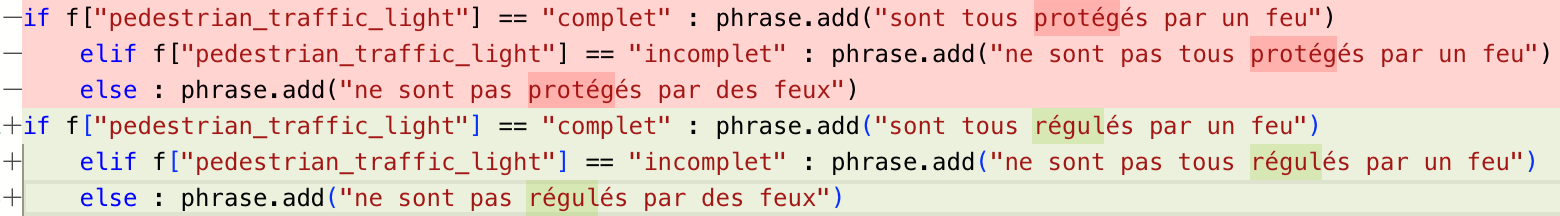
\includegraphics[width=\textwidth]{images/evaluation/pipeline/substitution.png}
        \caption[Exemple de substitution]{Exemple de substitution d'un terme dans le patron de description.}
        \label{fig:evaluation_reformulation_simple_substitution}
    \end{figure}
    \item \textbf{Modification du patron}: Une modification proposée par ID 32 sur le carrefour 1 propose de reformuler la description d'une branche en réagenceant les informations de voies par type et non par sens de circulation. Cette modification s'appuie sur les mêmes données que la description initiale, mais nécessite de modifier la structure de la phrase. De nouvelles règles de génération de texte devront être ajoutées au patron pour prendre en compte cette modification.
\end{itemize}
\end{samepage}

\subsubsection{Reformulation complexe}

Les reformulations complexes, au contraire des reformulations simples, ne s'appuient pas directement sur les formes de données déjà préparées mais sur la fusion de celles-ci pour proposer un texte plus élaboré. Elles s'opérent sur la transformation des données pour fusionner les informations nécessaires, sur l'implémentation du patron pour concevoir le nouveau texte en accord avec le nouveau schéma, et sur l'assemblage des descriptions pour transformer le plan en accord avec le nouveau texte (voir figure \ref{fig:evaluation_reformulation_complexe}).

\begin{figure}
    \centering
    
\includegraphics[width=\textwidth]{images/evaluation/pipeline/pipeline_reformulation_complexe.pdf}
    \caption[Reformulation complexe dans la chaîne de description]{La reformulation complexe agit sur de nombreuses brique de la chaîne de description.}
    \label{fig:evaluation_reformulation_complexe}
\end{figure}

\newpar{}

Une modification fournie par la réponse ID 52 sur le carrefour 1 propose de fusionner les descriptions des voies et des traversées en un seul paragraphe. Cette modification nécessite la réalisation de plusieurs étapes:

\begin{itemize}
    \item \textbf{Transformation des données}: Les tables des branches (table \ref{tab:experimentation_desc_branches}) et des traversées (table \ref{tab:experimentation_desc_traversées}) doivent être jointes en une seule table pour permettre leur description simultanée (voir table \ref{tab:evaluation_desc_branches}). La jointure s'opère dans la brique de transformation des données à l'aide des fonctions du \gls{sig} utilisé pour l'implémentation.
    \begin{table}[ht]
        \begin{center}
            \footnotesize
            \begin{tabular}{ | l | l | l | l | l |}
                \textbf{N° branche} & \textbf{Voies}& \makecell{\textbf{Nombre}\\\textbf{passages piéton}} & \makecell{\textbf{Feux}\\\textbf{piétons}} & …\\
                \hline
                2 & 
                \makecell{
                    \texttt[\\
                    \hspace{0.5cm}\texttt{\{}\\
                    \hspace{1cm}\texttt{"direction": "sortant",}\\
                    \hspace{1cm}\texttt{"lanes": [}\\
                    \hspace{1.5cm}\texttt{\{"number": 1, "type": "bus"\}}\\
                    \hspace{1cm}\texttt{]}\\
                    \hspace{0.5cm}\texttt{\},\{…\}}\\
                    \texttt]
                } & 1 & complet & …
            \end{tabular}
        \end{center}
        \caption[Jointure des tables branches et traversées]{Extrait de la jointure des tables des branches et des traversées pour la deuxième branche. Elle peut s'opérer à l'aide du numéro de branche qui joue le rôle d'identifiant unique.}
        \label{tab:evaluation_desc_branches}
    \end{table}
    \item \textbf{Implémentation du patron}: La nouvelle table de description des branches et des traversées ne dispose d'aucun patron de description. En accord avec le texte proposé par la réponse ID 52, un nouveau patron doit être implémenté pour générer le texte souhaité (voir figure \ref{fig:evaluation_patron_reformulation_complexe}).
    \begin{figure}[ht]
        \centering
        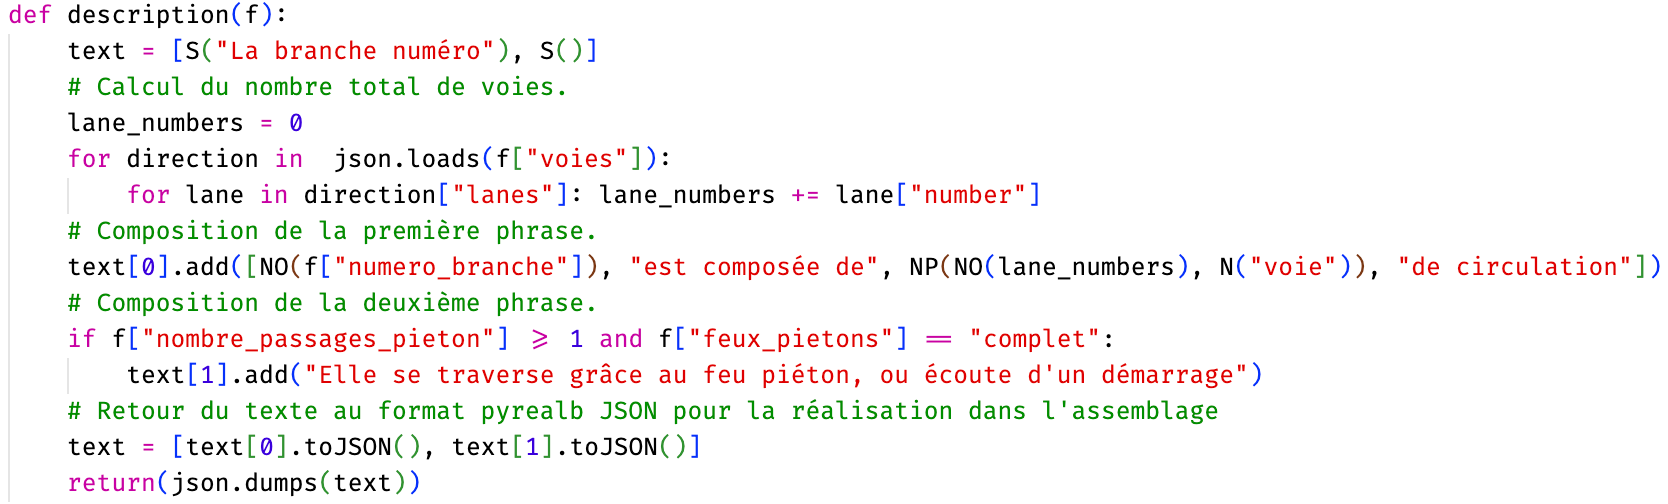
\includegraphics[width=\textwidth]{images/evaluation/pipeline/reformulation_complexe.png}
        \caption[Patron de description pour une reformulation complexe]{Exemple de patron de description permettant la description simultanée d'une branche et de sa traversée dans le cas d'une traversée simple. Seul le cas indiqué par la réponse ID 52 (présence d'une traversée et d'un feu piéton) est présenté ici.}
        \label{fig:evaluation_patron_reformulation_complexe}
    \end{figure}
    \item \textbf{Assemblage des descriptions}: La réponse ID 52 propose un plan remanié, où les parties dédiées à la description des branches et à la description des traversées sont remplacées par une unique partie décrivant les deux simultanément. L'étape d'assemblage doit donc être modifiée pour remplacer l'appel aux deux patrons précédents par le nouveau.
\end{itemize}

\newpage

\subsubsection{Nouvelle information sans ajout de données}

Formuler une nouvelle information sans ajout de données consiste à se reposer sur les entrées déjà disponibles dans la chaîne pour générer un nouveau texte contenant une information absente de la description d'origine. Cela signifie qu'il est nécessaire d'appliquer de nouveaux algorithmes aux données en entrées pour faire émerger ces informations. Cette dernière étape s'opère donc dans la transformation des données, puis dans l'implémentation du patron pour générer le nouveau texte en accord avec le nouveau schéma. L'assemblage des descriptions peut également être modifié si la nouvelle information nécessite de revoir la structure du plan de description (voir figure \ref{fig:evaluation_nouvelle_information_sans_ajout}).

\begin{figure}[ht]
    \centering
    
\includegraphics[width=\textwidth]{images/evaluation/pipeline/pipeline_reformulation_complexe.pdf}
    \caption[Formulation d'une nouvelle information sans ajout de données dans la chaîne de description]{La formulation d'une nouvelle information sans ajout de données agit sur les mêmes briques que la reformulation complexe. En revanche, des traitements algorithmiques plus complexes sont appliquées aux données d'entrées pour générer l'information nécessaire.}
    \label{fig:evaluation_nouvelle_information_sans_ajout}
\end{figure}

\newpar{}

Une modification fournie par la réponse ID 39 sur le carrefour 1 propose d'ajouter des précisions sur les voies reliant deux branches (dites <<~voies de raccourci~>>, voir figure \ref{fig:evaluation_voie_de_raccourci}) aux paragraphes de description des branches.

\begin{figure}[ht]
    \centering
    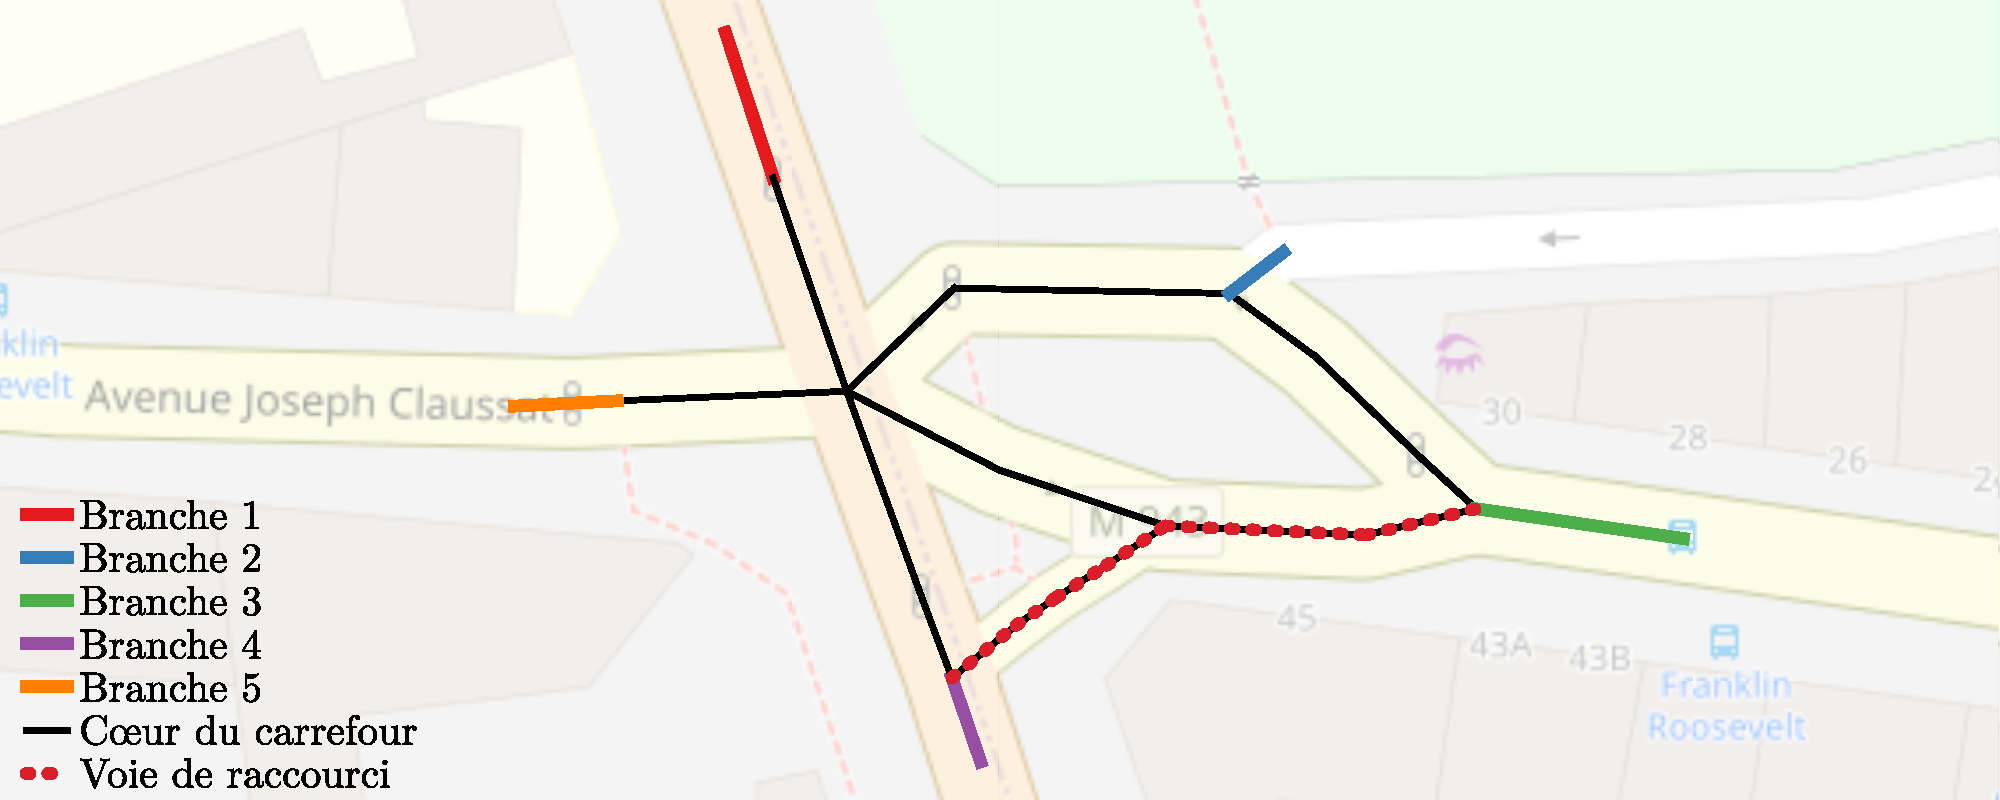
\includegraphics[width=\textwidth]{images/evaluation/pipeline/voie_raccourci.pdf}
    \caption[Une <<~voie de raccourci~>> dans un carrefour]{Une <<~voie de raccourci~>> permet de relier ensemble deux branches en restant sur l'extérieur du carrefour.}
    \label{fig:evaluation_voie_de_raccourci}
\end{figure}

\newpar{}

Les étapes d'implémententation de cette modification sont les suivantes:

\begin{itemize}
    \item \textbf{Transformation des données}: Les voies de raccourci sont présentes dans le graphe du carrefour généré par crseg, mais pas sémantiquement délimitées ni par crseg ni par crmodel. Une étape au sein du \gls{sig} est donc ici nécessaire pour calculer si un segment routier permet de relier deux branches sans passer par le centre du carrefour. Dans l'exemple de modification du schéma de la table des branches en figure \ref{tab:eval_voie_de_raccourci}, l'information est intégrée dans le champ de description des voies.
    \begin{table}[ht]
        \begin{center}
            \footnotesize
            \begin{tabular}{ | l | l | l | }
                \makecell{\textbf{N°}\\\textbf{branche}} & \textbf{Nom} & \textbf{Voies}\\
                \hline
                3 &
                \makecell{
                    \texttt{\{}\\
                    \hspace{0.5cm}\texttt{\{"type": "avenue"\}},\\
                    \hspace{0.5cm}\texttt{\{"name": "Roosevelt"\}}\\
                    \texttt\}
                } &
                \makecell{
                    \texttt[\\
                    \hspace{0.5cm}\texttt{\{}\\
                    \hspace{1cm}\texttt{"direction": "entrant",}\\
                    \hspace{1cm}\texttt{"lanes": [\{}\\
                    \hspace{1.5cm}\texttt{"number": 1, "type": "circulation",}\\
                    \hspace{1.5cm}\texttt{"shortlink\_from": 4,}\texttt{"shortlink\_to": null}\\
                    \hspace{1cm}\texttt{\}]}\\
                    \hspace{0.5cm}\texttt\}\\
                    \texttt]
                }\\
                \hline
                4 & 
                \makecell{
                    \texttt{\{}\\
                    \hspace{0.5cm}\texttt{\{"type": "boulevard"\}},\\
                    \hspace{0.5cm}\texttt{\{"name": "Berthelot"\}}\\
                    \texttt\}
                } &
                \makecell{
                    \texttt[\\
                    \hspace{0.5cm}\texttt{\{}\\
                    \hspace{1cm}\texttt{"direction": "sortant",}\\
                    \hspace{1cm}\texttt{"lanes": [\{}\\
                    \hspace{1.5cm}\texttt{"number": 2, "type": "circulation",}\\
                    \hspace{1.5cm}\texttt{"shortlink\_from": null,}\texttt{"shortlink\_to": 3}\\
                    \hspace{1cm}\texttt{\}]}\\
                    \hspace{0.5cm}\texttt{\},\{…\}}\\
                    \texttt]
                }
            \end{tabular}
        \end{center}
        \caption[Intégration des voies de raccourci au schéma des branches]{Exemple d'intégration de l'information de présence de la voie de raccourci du carrefour en en figure \ref{fig:evaluation_voie_de_raccourci}. Sur la branche 3, l'attribut shortlink\_from permet d'indiquer de quelle branche les véhicules proviennent. Sur la branche 4, l'attribut shortlink\_to permet d'indiquer vers quelle branche les véhicules se dirigent.}
        \label{tab:eval_voie_de_raccourci}
    \end{table}
    \item \textbf{Modification du patron}: Le patron décrivant une branche doit être modifié pour refléter la présence d'une voie de raccourci (voir figure \ref{fig:evaluation_patron_voie_de_raccourci}).
    \begin{figure}[H]
        \centering
        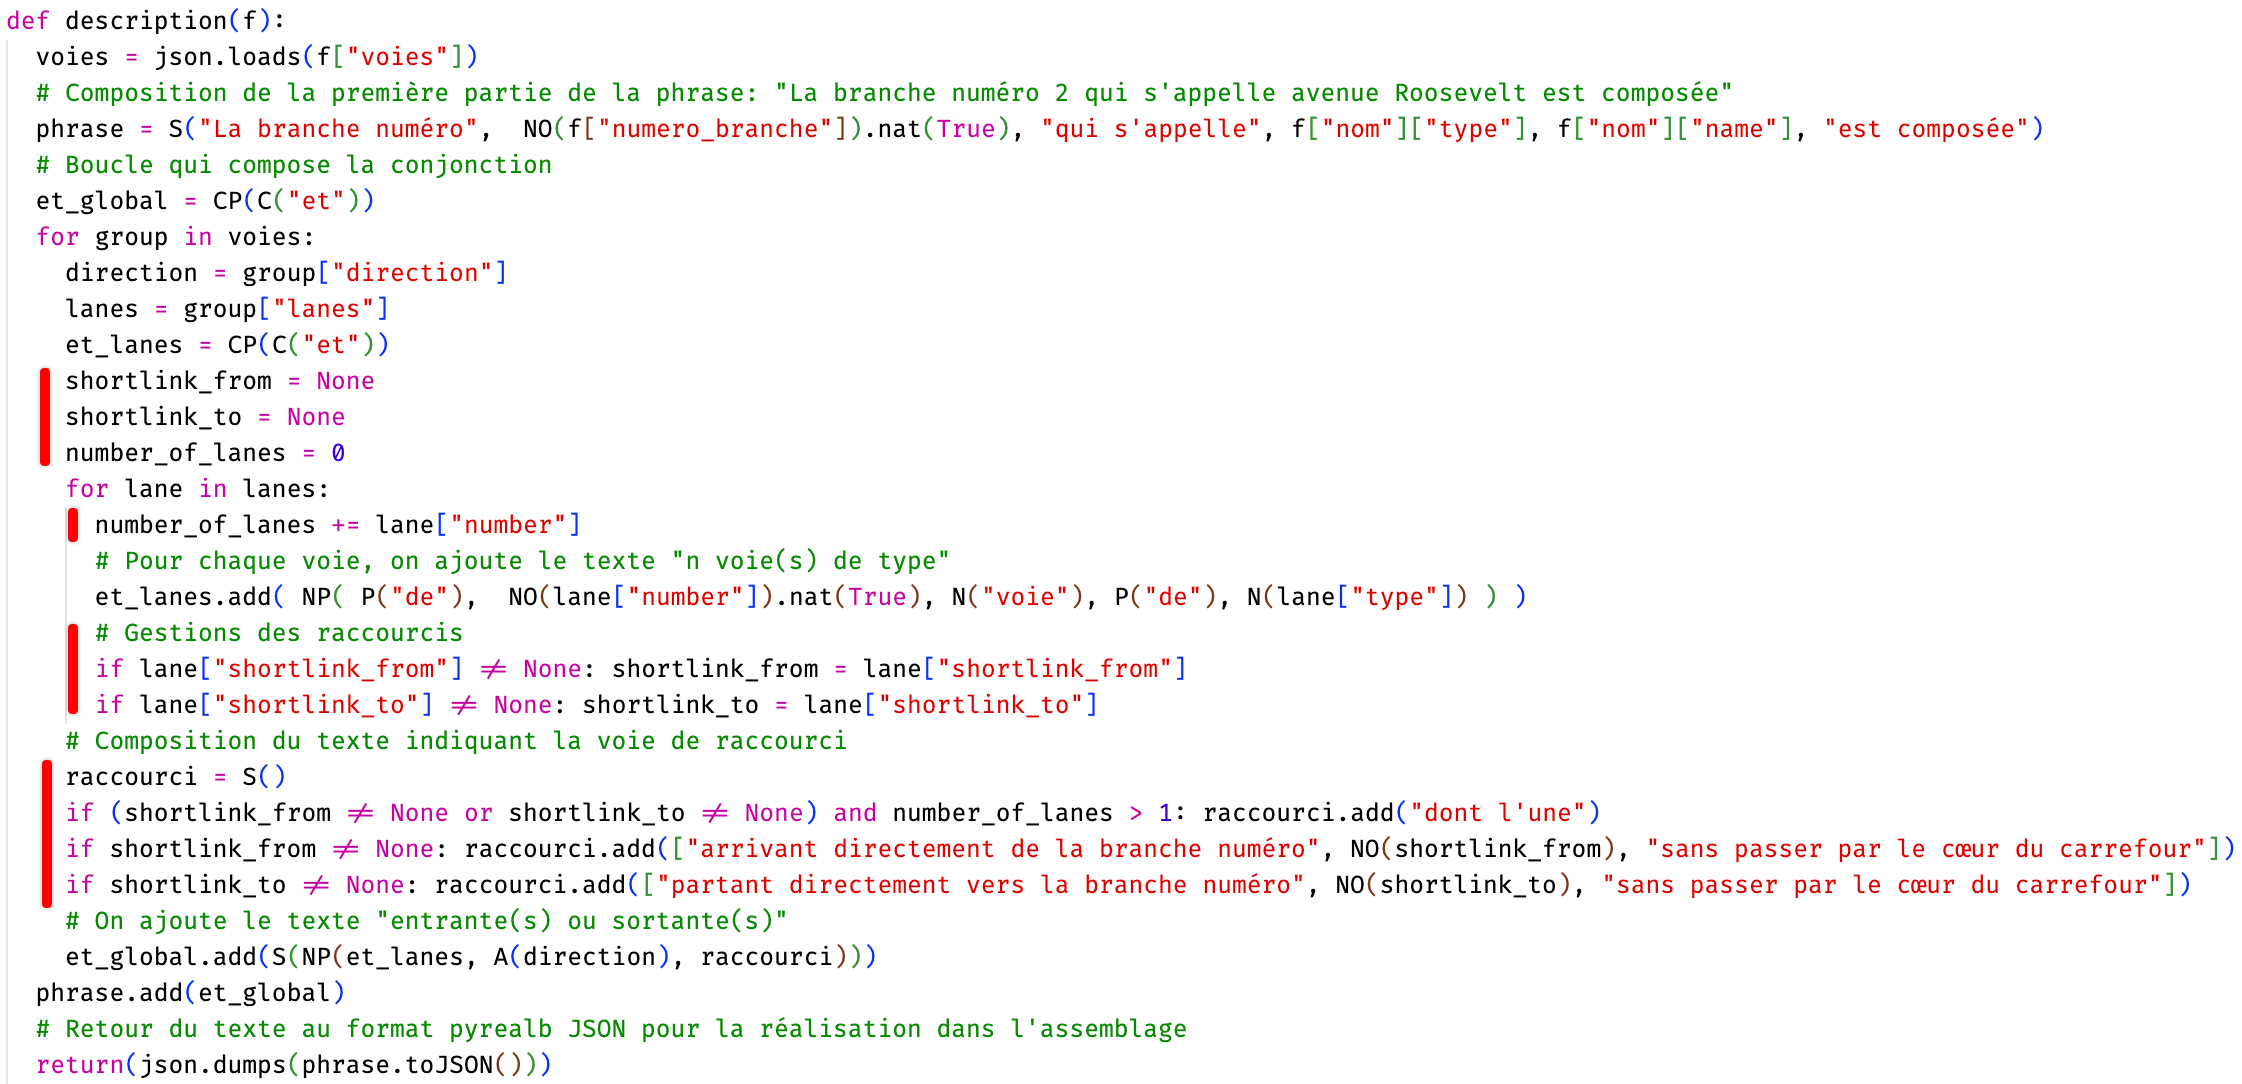
\includegraphics[width=\textwidth]{images/evaluation/pipeline/nouvelle_info.png}
        \caption[Patron modifié pour intégrer les <<~voies de raccourci~>>]{Le patron de description de branche est ici modifié (lignes identifiées par une ligne rouge) pour intégrer la description d'une <<~voie de raccourci~>> si elle est présente.}
        \label{fig:evaluation_patron_voie_de_raccourci}
    \end{figure}
\end{itemize}

\newpage

\subsubsection{Nouvelle information avec ajout de données}

Formuler une nouvelle information avec ajout de données consiste à ajouter de nouvelles données en entrée pour générer un nouveau texte contenant une information absente de la description d'origine. Cela signifie qu'il est nécessaire, à l'instar du processus présenté en partie \ref{sec:implementation_segmentation}, de les transformer pour les adapter à la description que l'on souhaite en faire. Il peut par ailleurs être nécessaire de les fusionner aux données originellement présente en entrée de la chaîne. Ces étapes peuvent  donc s'opérer sur l'intégralité de la chaîne, de la transformation des données à l'assemblage des descriptions (voir figure \ref{fig:evaluation_nouvelle_information_avec_ajout}).

\begin{figure}[ht]
    \centering
    
\includegraphics[width=\textwidth]{images/evaluation/pipeline/pipeline_ajout_donnees.pdf}
    \caption[Formulation d'une nouvelle information avec ajout de donnée dans la chaîne de description]{La formulation d'une nouvelle information avec ajout de données agit sur les mêmes briques que la catégorie précédente. En revanche, l'ajout de nouvelles données implique de revoir l'intégralité de la chaîne.}
    \label{fig:evaluation_nouvelle_information_avec_ajout}
\end{figure}

\newpar{}

Des modifications fournie par les réponses ID 52 et ID 56 proposent d'ajouter des informations sur les feux sonores aux descriptions des traversées. Ces informations sont présentes dans \gls{osm} mais ne sont pas intégrées à CrModel. Il est donc nécessaire de les acquérir et de les traiter pour les intégrer à la description. Les étapes d'implémentation de cette modification sont détaillées ci-dessous:

\begin{itemize}
    \item \textbf{Intégration des données}: Les feux sonores sont présents dans \gls{osm} sous la forme d'une clé (\osmkey{traffic\_signals:sound}) sur les passages piéton. Il est possible de télécharger les passages piéton sur la zone d'intérêt pour les intégrer au SIG.
    \item \textbf{Transformation des données}: crmodel conserve pour chaque objet issu d'\gls{osm} les identifiants qui lui sont associées. Il est donc possible de réaliser une jointure entre les données nouvellement importées et les traversées existantes pour ajouter un champ à la couche indiquant la présence ou l'absence de feux sonores sur la traversée.
    \item \textbf{Modification du patron}: Le patron décrivant une traversée doit être modifié en accord avec le nouveau champ créé pour refléter la présence ou l'absence de feux sonores.
\end{itemize}

\section{Conclusion du chapitre}

Dans ce chapitre, nous avons présenté les évaluations statistiques de crseg et crmodel, les deux outils développés dans le cadre de cette thèse pour générer un modèle de carrefour,  et nous avons vu que leur résultat était très dépendant de la qualité des données \gls{osm}. 

\newpar{}

Nous avons également réalisé une évaluation du canevas de description en confrontant sa modularité aux besoins exprimés par les professionnels de la déficience visuelle. Ces besoins ont été recueillis au sein d'une enquête visant à adapter une description à leurs pratiques. Les réponses ont été étiquetés par type de modification et nous avons, pour chaque type, déterminé les étapes nécessaires à l'intégration de ces modifications au sein du canevas. Nous avons vu à travers quelques exemple que celui-ci est suffisamment modulaire pour permettre d'intégrer certaines modifications proposées, sous réserve de la disponibilité des données nécessaires à leur réalisation, et de la mise en place de nouveaux traitements et patrons de descriptions. La complexité des modifications à réaliser pour modifier la description est en fait très variable, et dépend fortement de la nature de l'information à ajouter ou à modifier.